

% ToDo: Video-centric and approaches for video and images.
\chapter{Robot Learning}
\label{chap:RobotLearningApproaches}
\minitoc
In this Chapter, we will focus more closely on the various distinct but interrelated categories of approaches, which use the objectives from Chapter~\ref{chap:RobotLearningObjectivesForUnderstandingDemonstrationVideos} to learn a coherent robot model \cite{Eze2024LearningBW}. The main focus lies on the intersection of \ac{LfV} and \ac{RL}, highlighting how video-based learning can enhance \ac{RL} algorithms and enable more efficient policy learning from visual data. Finally we give a brief introduction to \ac{VLA} models, which is currently the peak of research in the field of video-based robot learning.

\section{Perception and Representation Learning}
The foundation of video-based robot learning relies on the ability to extract task relevant information from visual data and translate it into robot-compatible representations. Robust perceptual and representational foundations are crucial for bridging the gap between human demonstrations and robot execution and enables agents to understand what matters in a video and how to replicate it \cite{Eze2024LearningBW}. 
% these foundations enable agents to understand what matters in a task and how to replicate it.
%  By learning meaningful representations of the environment, understanding object affordances and human-object interactions, recognizing human actions and activities and modeling 3D hand movements, robots can acquire complex manipulation skills from videos. These foundational capabilities enable robots to interpret dynamic scenes, extract task-relevant features and generalize across varying environments and embodiments, ultimately facilitating more effective \ac{IL} and skill acquisition.

This section is divided into:
\begin{enumerate}
    \item \textit{Feature Extraction Methods} which focus on extracting meaningful structured spatio-temporal features from video data, including spatial understanding, temporal modeling and geometry-aware representations \cite{Eze2024LearningBW}.
    \item \textit{Domain Bridging Approaches} which aim to reduce the gap between different domains, such as sim-to-real or human-to-robot transfer by translating visual or contextual information from videos into robot-compatible representations \cite{Eze2024LearningBW}.
\end{enumerate}



\subsection{Feature Extraction Methods}
Feature extraction methods aim to obtain task-relevant information from visual demonstrations, ranging from holistic scene understanding to fine-grained motion structure. In robotic imitation learning, these approaches provide the perceptual foundation for mapping visual observations to robot actions \cite{Eze2024LearningBW}.

% The goal of feature extraction is to obtain task-relevant information from raw video data, ranging from holistic visual features (e.g., object masks, hand-object interactions) to fine-grained structural cues (e.g., joint angles, keypoint trajectories). To achieve this, the field has developed two complementary strategies: CNN-based feature extraction and pose/keypoint detection.

\begin{figure}
	\centering
	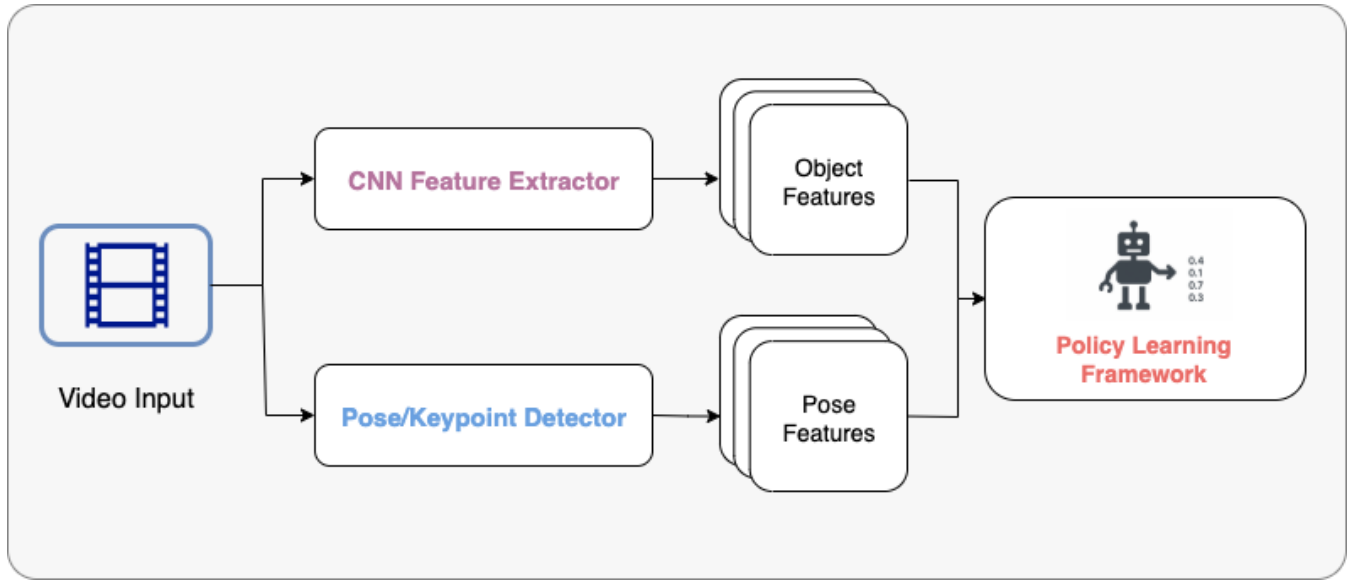
\includegraphics[width=1.0\linewidth]{./chapter6/media/ApproachesFeatureExtraction}
	\caption[Feature Extraction: Methods Overview]{Feature Extraction: Methods Overview. Image source: \cite{Eze2024LearningBW}.}
	\label{fig:ApproachesFeatureExtraction}
\end{figure}

\begin{itemize}
    \item \textbf{\acs{CNN}-based Feature Extraction:} \acp{CNN} excel at spatial feature extraction and learn spatio-temporal representations directly from raw pixels \cite{Qiu2017LearningSR}. These approaches are widely used for detecting objects, segmenting interaction regions and modeling hand-object relationships from demonstrations \cite{Lee2017LearningRA, Zhang2019LearningCA, Zhang2019AnOA}. \ac{CNN}-based pipelines form the foundation of many Robot Learning systems and support the direct mapping of raw visual observations to robot actions \cite{Eze2024LearningBW}.
    \item \textbf{Pose and Keypoint Detection:} In contrast, pose and keypoint-based methods focus on extracting structured skeletal motion representations such as body joints, hand poses, fingertips, or object centers. % such as elbows, wrists, fingertips, or
    Instead of analyzing the entire image equally, these methods identify important points of the human body or hand or object locations and track how they move over time \cite{Eze2024LearningBW}. This helps the system understand how a person moves, how body parts relate to each other and how humans interact with objects during a task . Pose-based methods are particularly useful for retargeting human demonstrations to robot kinematics, since the reconstructed joint trajectories can be mapped to robot motions \cite{Sivakumar2022RoboticTL, Bahl2022HumantoRobotII}. For example, several approaches reconstruct 3D human poses from monocular videos and transfer the resulting trajectories into robot-compatible action representations for policy learning \cite{Sivakumar2022RoboticTL, Deng2023AHC, Zhu2024VisionbasedMF}.
\end{itemize}


These pose-based methods complement \ac{CNN}-based pipelines—while \acp{CNN} extract dense, holistic features, pose and keypoint detection supplies structured, low-dimensional skeletal motion cues that ease embodiment alignment and improve robustness in human-to-robot transfer tasks. Both methods can provide valuable information for downstream policy learning. 
% ToDo:
%  and many systems combine them to leverage their respective strengths.

Feature extraction methods are generally data-efficient and flexible, making them well-suited for learning from large-scale unlabeled video data and producing interpretable representations. They integrate effectively with \ac{RL} and \ac{IL} frameworks, particularly for modeling perception-driven control and effective for action parsing and object-centric manipulation tasks. 

\textit{Challenges.} Nevertheless, these methods still struggle with sim-to-real or human-to-robot embodiment transfer, long-horizon and high-level policy reasoning or domain shift between human demonstrations and robotic execution \cite{Eze2024LearningBW}.





\subsection{Domain Bridging via Translation}
This category addresses the domain shift—the mismatch in human and robot embodiment, visual appearance and context—between human demonstration videos and robot execution. Translation techniques convert visual and contextual data into robot-compatible representations, such that human demonstrations become more directly usable for robot learning \cite{Eze2024LearningBW}. 
% These approaches are crucial for enabling sim-to-real transfer and human-to-robot \ac{IL}, as they reduce the gap between the source (human videos) and target (robot policies) domains.

\begin{itemize}
    \item \textbf{Image Translation:}
    Image Translation techniques focus on aligning visual appearance between human and robot domains. The main idea is to translate human videos directly into a robot-like visual style or make simulated robot data more realistic. For example, mapping the visual appearance of a human arm to the robot arm or the human hand to the robot gripper. This allows robots to learn from human demonstrations while observing them in a visually consistent format \cite{Eze2024LearningBW}.

    A common approach is based on \acp{GAN}, which consist of two competing models: A generator that produces the translated robot images and a discriminator that tries to distinguish between real and generated robot images. The goal is for the generator to generate robot images that look realistic enough that the discriminator cannot distinguish them from real ones. Through this competition, the generator learns to produce increasingly realistic images that match the target domain \cite{Isola2016ImagetoImageTW, Zhu2017TowardMI, Liu2017UnsupervisedIT}. CycleGAN based approaches extend this idea by adding a cycle-consistency constraint, meaning that translating an image from domain A to B and back to A should reconstruct the original image \cite{Zhu2017UnpairedIT}. This allows learning translation between human and robot domains without requiring paired examples.

    % ToDo: Quellen nicht vollständig
    Based on these principles, early \ac{GAN}-based methods \cite{Isola2016ImagetoImageTW, Zhu2017TowardMI, Liu2017UnsupervisedIT} improved the realism of training data and supported better generalization to robot manipulation tasks \cite{erdei2024image}. More advanced approaches use conditional \acp{GAN} to predict intermediate visual goals from demonstrations, which are then executed by a separate low-level controller, effectively separating perception from control \cite{Sharma2019ThirdPersonVI}. Other methods, such as AVID \cite{Smith2019AVIDLM}, apply CycleGAN to directly translate human videos into robot-like images, using the resulting frames as reward signals for \ac{RL}. More recent approaches extend this idea with transformer-based architectures, bidirectional translation, meta-learning and \ac{RL}, enabling fast adaptation to new tasks with minimal demonstrations \cite{Dasari2020TransformersFO, Li2022MetaImitationLB}.


    \item \textbf{Context Translation:}
    Context translation methods extend beyond the alignment of visual appearance and focus on transferring skills across varying tasks, environments, viewpoints and object configurations \cite{Liu2023CEILGC}. The main goal is to enable robots to generalize learned behaviors to new contexts by capturing the underlying structure of a task or the relationships between different elements in the environment rather than relying on specific visual conditions. In short terms, the idea is to learn ``what is being done'' rather than ``how it looks like'' in a particular scene.
    % Context Translation techniques transfer skills across broader contextual variables, such as tasks, environments, viewpoints and objects. These methods aim to generalize learned behaviors to new situations by understanding the underlying structure of the task and the relationships between different elements in the environment.

    Early approaches learn from paired demonstrations collected in different environments, where the same action is shown under varying contexts. These models learn to translate how a skill appears across settings, enabling robots to reproduce the same behavior in novel environments through \ac{RL} \cite{Liu2017ImitationFO}. Later methods improve robustness by learning context-agnostic task representations that are combined with multi-modal inverse dynamics models $p^{-1}(\hat{a}_t \mid o_t, c_t, o_{t+1}, c_{t+1})$, by integrating RGB ($o$) and depth (represented as conditional modality $c$) information as the input. These systems achieve more stable action prediction across changes in viewpoint and object layout \cite{Yang2020CrosscontextVI}.

    % ToDo:
    % context-agnostic task representations = independent of specific visual conditions such as camera viewpoint, background, or object placement

    More recent approaches focus on scalability through unsupervised learning. The Learning by Watching (LbW) framework \cite{Xiong2021LearningBW} combines video translation models with unsupervised keypoint extraction to map human demonstrations into robot domains without task-specific supervision. The resulting structured keypoint representations are then used as inputs for \ac{RL}, enabling imitation under varying contextual conditions while reducing the need for expert-labeled data.
\end{itemize}



\paragraph{Example}
Learning goal: The Robot should learn to bake a cake from a YouTube video
\begin{enumerate}
    \item \textbf{Feature Extraction:} 
    \begin{itemize}
        \item The robot uses \textit{\acs{CNN}-based feature extraction} to identify the kitchen counter, the ingredients and the tools.
        \item It also applies \textit{pose and keypoint detection} to track precise hand movements, such as how the person exactly grips the whisk or the angle of the hand when pouring.
    \end{itemize}


    \item \textbf{Domain Bridging:} 
    \begin{itemize} 
        \item The robot applies \textit{image translation} to make the human's hand look like the robot's gripper in the video.
        \item It also uses \textit{context translation} to adapt the skill learned in a brightly lit human kitchen to be successfully executed in the robot's dimly lit, specialized lab environment, effectively adapting the action plan to the novel context.
    \end{itemize} 
\end{enumerate}


\paragraph{Summary \& Limitations}
Image and context translation provide complementary approaches to bridging domain gaps between training data and real-world execution. Image translation focuses on visual alignment, making human demonstrations look like robot observations, while context translation captures the underlying task structure and relationships that enable generalization across varying environments and embodiments \cite{Eze2024LearningBW}. 

\textit{Challenges.} However, methods still lack at precise action alignment, translation artifacts and managing mismatches between embodiment alignment \cite{Eze2024LearningBW}.






\section{Reinforcement Learning}
% RL enables robots to acquire manipulation skills via trial-and-error guided by reward signals. By learning from interaction with the environment, RL can optimize policies for complex tasks. However, RL typically requires large amounts of interaction data, which can be impractical for real-world robotic applications. Simulation data can be used, but requires some engeneering effort too. Leveraging video data to extract useful information for RL can significantly improve performance and learning efficiency to require less amounts of interaction data.

\ac{RL} enables robots to acquire manipulation skills through trial-and-error interaction guided by reward signals. By continuously interacting with the environment, RL can optimize policies for complex and long-horizon tasks that are difficult to solve with purely supervised approaches. 

In the context of \ac{LfV}, RL approaches often combine exploratory learning with structured information extracted from human demonstrations \cite{Eze2024LearningBW}. Rather than forming strictly separated categories, the following approaches represent complementary strategies that can be integrated within broader RL frameworks, see \autoref{fig:RLApproaches}.

\begin{figure}[!ht]
	\centering
	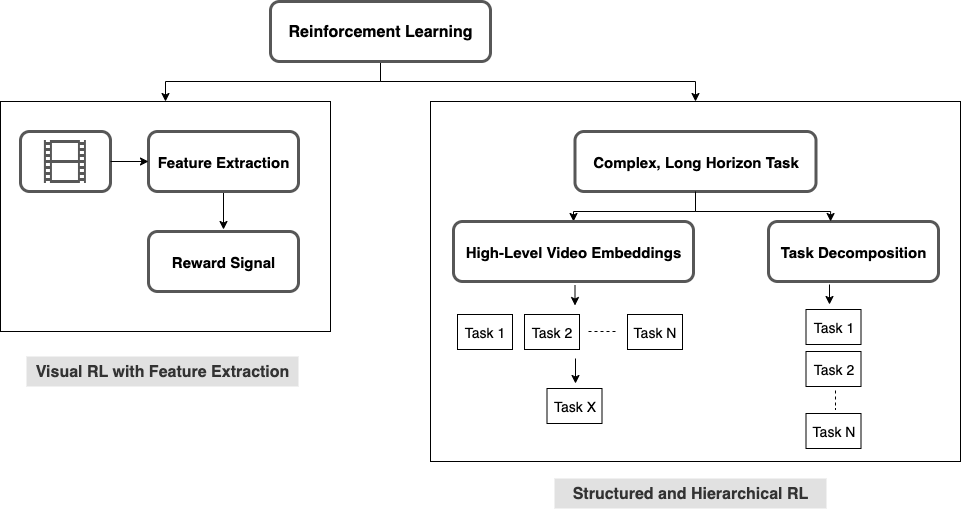
\includegraphics[width=1.0\linewidth]{./chapter6/media/RLApproaches}
	\caption[Reinforcement Learning: General overview of video-based robot learning paradigms.]{Reinforcement Learning: General overview of video-based robot learning paradigms. Image source: \cite{Eze2024LearningBW}.}
	\label{fig:RLApproaches}
\end{figure}


% ToDo: Use examples on my PowerPoint in the RL section
\begin{itemize}
    \item \textbf{Visual RL with Feature Extraction}
    
    Visual RL with feature extraction focuses on deriving meaningful visual representations on video data, using them to guide \ac{RL}. Video demonstrations are transformed into structured training signals, such as object trajectories, motion representations, latent embeddings, or dense reward functions, which help RL agents learn more efficiently from limited interaction data \cite{Schmeckpeper2020ReinforcementLW, Petrik2020LearningOM, Zorina2021LearningTM}. These approaches reduce the need for manually engineered rewards and improve policy learning by grounding exploration in semantically meaningful visual features.

% Combine RL's exploration and optimization power with rich perceptual inputs from videos.
% Goal: Transform video demonstrations into usable training signals for RL policies.
% Leveraging these representations to generate dense reward signals for RL policies
    \item \textbf{Structured and Hierarchical RL} 
    
    Structured and hierarchical RL approaches decompose complex tasks into reusable skills, subtasks, or high-level goals. Instead of learning a single monolithic policy, the agent learns hierarchical representations that separate high-level planning from low-level control. Video data can be used to learn task embeddings, latent skills, or subgoal representations that enable multi-task learning, long-horizon reasoning and improved generalization across manipulation tasks \cite{Xu2017NeuralTP, Mees2019AdversarialSN, ChaneSane2023LearningVP}.

    In particular, hierarchical and multi-task RL frameworks enable the reuse of learned skills and improve generalization across diverse environments.
\end{itemize}

% A major strength of \ac{RL} lies in its ability to solve complex, long-horizon manipulation tasks through interaction-driven optimization. In particular, hierarchical and multi-task RL frameworks enable the reuse of learned skills and improve generalization across diverse environments
\textit{Challenges.} \ac{RL} typically requires large amounts of interaction data and carefully designed reward functions, making real-world robotic training expensive and time-consuming \cite{Eze2024LearningBW}. While simulation environments can alleviate this issue, they often require substantial engineering effort and suffer from sim-to-real transfer challenges. Leveraging information extracted from large-scale video data can significantly improve the data efficiency, robustness and generalization capabilities of \ac{RL} systems \cite{McCarthy_2025}.


\section{Imitation Learning}

\subsection{Idea Behind Imitation Learning} 
When we want to learn a new skill, we often turn to how-to videos. We learn the new skill through speech instructions and visual observations in the video \cite{Jain2024Vid2RobotEV}. The same principle is now to be applied to robots through \ac{IL}.

Visual Imitation Learning ...
\begin{itemize}
    \item is ideal for teaching tasks that are difficult or impossible to describe in words.
    \item allows robots to infer tasks from expert demonstrations in different environments than the robot.
    \item can be more data efficient than \ac{RL}, especially in high-dimensional state spaces, like a complex robot environment. 
    \item can leverage large datasets of human demonstrations, which are often easier to collect than expert demonstrations in the specific domain \cite{Jain2024Vid2RobotEV}.
\end{itemize}

% \texttt{Problems in RL:}
In \ac{RL} a task is commonly defined through a reward function, which assigns a high reward to desirable behavior and a low reward to undesirable behavior \cite{sutton2018reinforcement}. However, designing good reward functions is challenging for every task and many methods based on computer vision rely on annotated demonstrations in every new environment \cite{McCarthy_2025}. \ac{IL} allows us to learn complex behaviors that are difficult to specify through a reward function, or it can help us to define a good adaptive reward function for \ac{RL}.


\subsection{Research Directions in Imitation Learning}
\ac{IL} is one of the promising directions for learning robot policies from videos. It enables robots to acquire skills by directly mimicking actions observed in human or robot demonstrations, without the need for explicit reward functions or extensive trial-and-error interaction. \ac{IL} policies can be more sample-efficient and often have a better generalization than pure \ac{RL} policies, as they leverage the rich information contained in demonstrations to guide policy learning \cite{Eze2024LearningBW}. 
% By learning from videos, robots can acquire different behaviors and generalize across diverse tasks and environments, reducing the need for hand-crafted reward functions and extensive environment interactions.
\ac{IL} is divided into the subcategories Bahavior Cloning and Learning from Videos/Observation, see Section~\ref{sec:ImitationLearning}.


% ToDo: Methods
Learning from Videos/Observation approaches can be formulated as an inverse \ac{RL} problem, where the goal is to infer the underlying reward function that explains the observed behavior in the video. Once this cost function is recovered, a policy can be optimized to minimize the predicted cost, thereby reproducing the expert's behaviour \cite{Eze2024LearningBW, Torabi2018GenerativeAI}.
Generative Adversarial Imitation from Observation (GAIfO) \cite{Torabi2018GenerativeAI} employs a generative adversarial setup where a discriminator is trained to differentiate between state transitions coming from expert demonstrations and those generated by the robot's current policy. Simultaneously, the robot policy learns to produce transitions that the discriminator cannot distinguish from expert data, thereby matching the observed dynamics of the expert. 
% This approach provides a more scalable and action-free alternative to traditional IRL, making it well-suited for learning from raw human video data.
This is achieved without any explicit action labels and offers a more scalable alternative to traditional inverse \ac{RL} \cite{Eze2024LearningBW}.
% ,  making it well-suited for learning from raw human video data.


% Beyond these main categories, several complementary approaches have been developed to further enhance the capabilities of \ac{IL} from videos. 
In addition to these main categories, several complementary approaches have been developed to further enhance the capabilities of \ac{IL} from videos \cite{Eze2024LearningBW}.

\paragraph{Meta- \& Few-Shot Imitation Learning}
Meta- and Few-Shot \ac{IL} approaches focuses on improving generalization capabilities by training on diverse tasks so that robots can quickly adapt to novel tasks from only a handful of demonstrations \cite{Eze2024LearningBW, Finn2017ModelAgnosticMF, Song2022ACS}.
\begin{itemize}
    \item \textbf{Few-shot Learning:} Refers to a broad approach in which models can make accurate predictions using only a small number of examples. It is a subcategory of N-shot learning and includes One-shot learning (learning from a single example) and Zero-shot learning (no examples needed). In practice, few-shot learning often leverages techniques such as meta-learning, transfer learning, data augmentation, or data generation methods,e.g. using generative \ac{AI}. Combinations of these approaches are also common \cite{Ghadirzadeh2021BayesianMF, Song2022ACS}.

    \item \textbf{Meta-Learning:} Also known as ``learning to learn'', describes the development of models that can achieve strong performance from a small amount of data or with very few training steps, thereby adapting efficiently to new tasks. More formally, Meta-Learning is a approach that aims to improve the learning ability of models by enabling them to learn from prior experiences and transfer that knowledge to new tasks. The main goal is to adapt the learning ability from humans. These algorithms are typically trained on a wide variety of different tasks, that the model can learn how to quickly adapt to new tasks \cite{Eze2024LearningBW, Ghadirzadeh2021BayesianMF, Song2022ACS}.
\end{itemize}

Few-shot learning refers to the ability to learn from a small number of examples, while meta-learning describes approaches for achieving this few-shot capability. 

\paragraph{Methods} 
Meta-learning approaches like Model-Agnostic Meta-Learning (MAML) have been applied to \ac{IL}, where policies are pre-trained on diverse tasks so that a single new demonstration suffices for adaptation \cite{Yu2018OneShotIF}.

% ToDo: Add examples from my Literatur 
% MOSAIC 

\paragraph{Cross-Domain \& Human-to-Robot Transfer}
Cross-domain and  human-to-robot transfer methods aim to achieve robust transfer from human video demonstrations to robot execution, addressing the challenges of embodiment differences and domain shift between human and robot data \cite{Eze2024LearningBW}. These approaches typically learn domain-invariant representations, intermediate action representations, or apply domain adaptation techniques to bridge the gap between human demonstrations and robot execution.
% ToDO: Quelle für den letzten Satz?

\paragraph{Methods.}
Multi-step task learning from human videos \cite{Goo2018OneShotLO} localizes human-demonstrated actions within supplemental videos and combines \ac{BC}, inverse \ac{RL} and \ac{RL} for accelerated policy refinement.

Watch, Try, Learn (WTL) \cite{Zhou2019WatchTL} combines visual meta-learning with binary feedback (success/failure). A robot first watches a human demonstration, then attempts to perform the task. After each attempt, it receives only a simple success or failure signal instead of a detailed reward. Using meta-learning, the robot rapidly updates its policy across a small number of such trials to refine its behavior. 
% This allows the robot to refine its behavior even when task success is rare or rewards are difficult to engineer.

Visual Entity Graphs (VEGs) \cite{Sieb2019GraphStructuredVI} models spatial and temporal relations between objects and actions using graph-based representations. By explicitly modelling how entities interact over time, the graph provides a structured, domain-invariant representation. This enables the robot to learn from a single demonstration: the graph abstracts away low-level visual differences between human and robot embodiments, allowing direct transfer of action-relevant relationships to the robot's own environment.


% ToDo Example ??: https://www.semanticscholar.org/paper/Hierarchical-Human-to-Robot-Imitation-Learning-for-Lin-Chen/54c3f1e7e8a830fb81fd5381c5b3970732bda2f6
% https://www.semanticscholar.org/paper/Adaptive-Video-Conditioned-Imitation-Learning-via-Lin-Chen/ef5c9be1161d01127366c2b9d20fe7378dadd413
% https://www.semanticscholar.org/paper/Bridging-Simulation-and-Reality%3A-Cross-Domain-with-Tang-Pang/e591fec42e66f5ac44887cf0d58c88d1eea625c5





\section{Hybrid Approaches}
\ac{RL} is a powerful approach for learning complex tasks, as it enables agents to improve their behavior through interaction with the environment \cite{Eze2024LearningBW}. However, it can be sample inefficient and may require a large number of interactions to learn an effective policy, especially in high-dimensional state and action spaces. Therefore, it is often combined with other learning paradigms, such as supervised learning or \ac{IL}, in order to leverage their complementary strengths and improve overall performance \cite{Eze2024LearningBW, McCarthy_2025}.

\ac{IL} generally refers to a family of methods and techniques that enable learning from demonstrations. Two important approaches in this context are \ac{BC} and \ac{LfV}, which differ primarily in the type of data they utilize. \ac{BC} relies on annotated demonstrations, where state-action pairs are available and learns a policy directly via supervised learning. In contrast, \ac{LfV} aims to infer actions from unannotated video observations, where in the most casses only visual information is provided.

Hybrid approaches combine \ac{RL}, \ac{IL} and complementary techniques to overcome the limitations of relying on a single learning paradigm, see Figure~\ref{fig:overviewroboticlearning}. The central motivation is to integrate the sample efficiency and structured guidance of \ac{IL} with the exploration and optimization strengths of \ac{RL} \cite{Eze2024LearningBW} \cite{Ramachandruni2020AttentiveTS}. By leveraging multiple training strategies simultaneously, hybrid methods aim to improve data efficiency, robustness and generalization in complex robotic manipulation tasks.

\begin{figure}
	\centering
	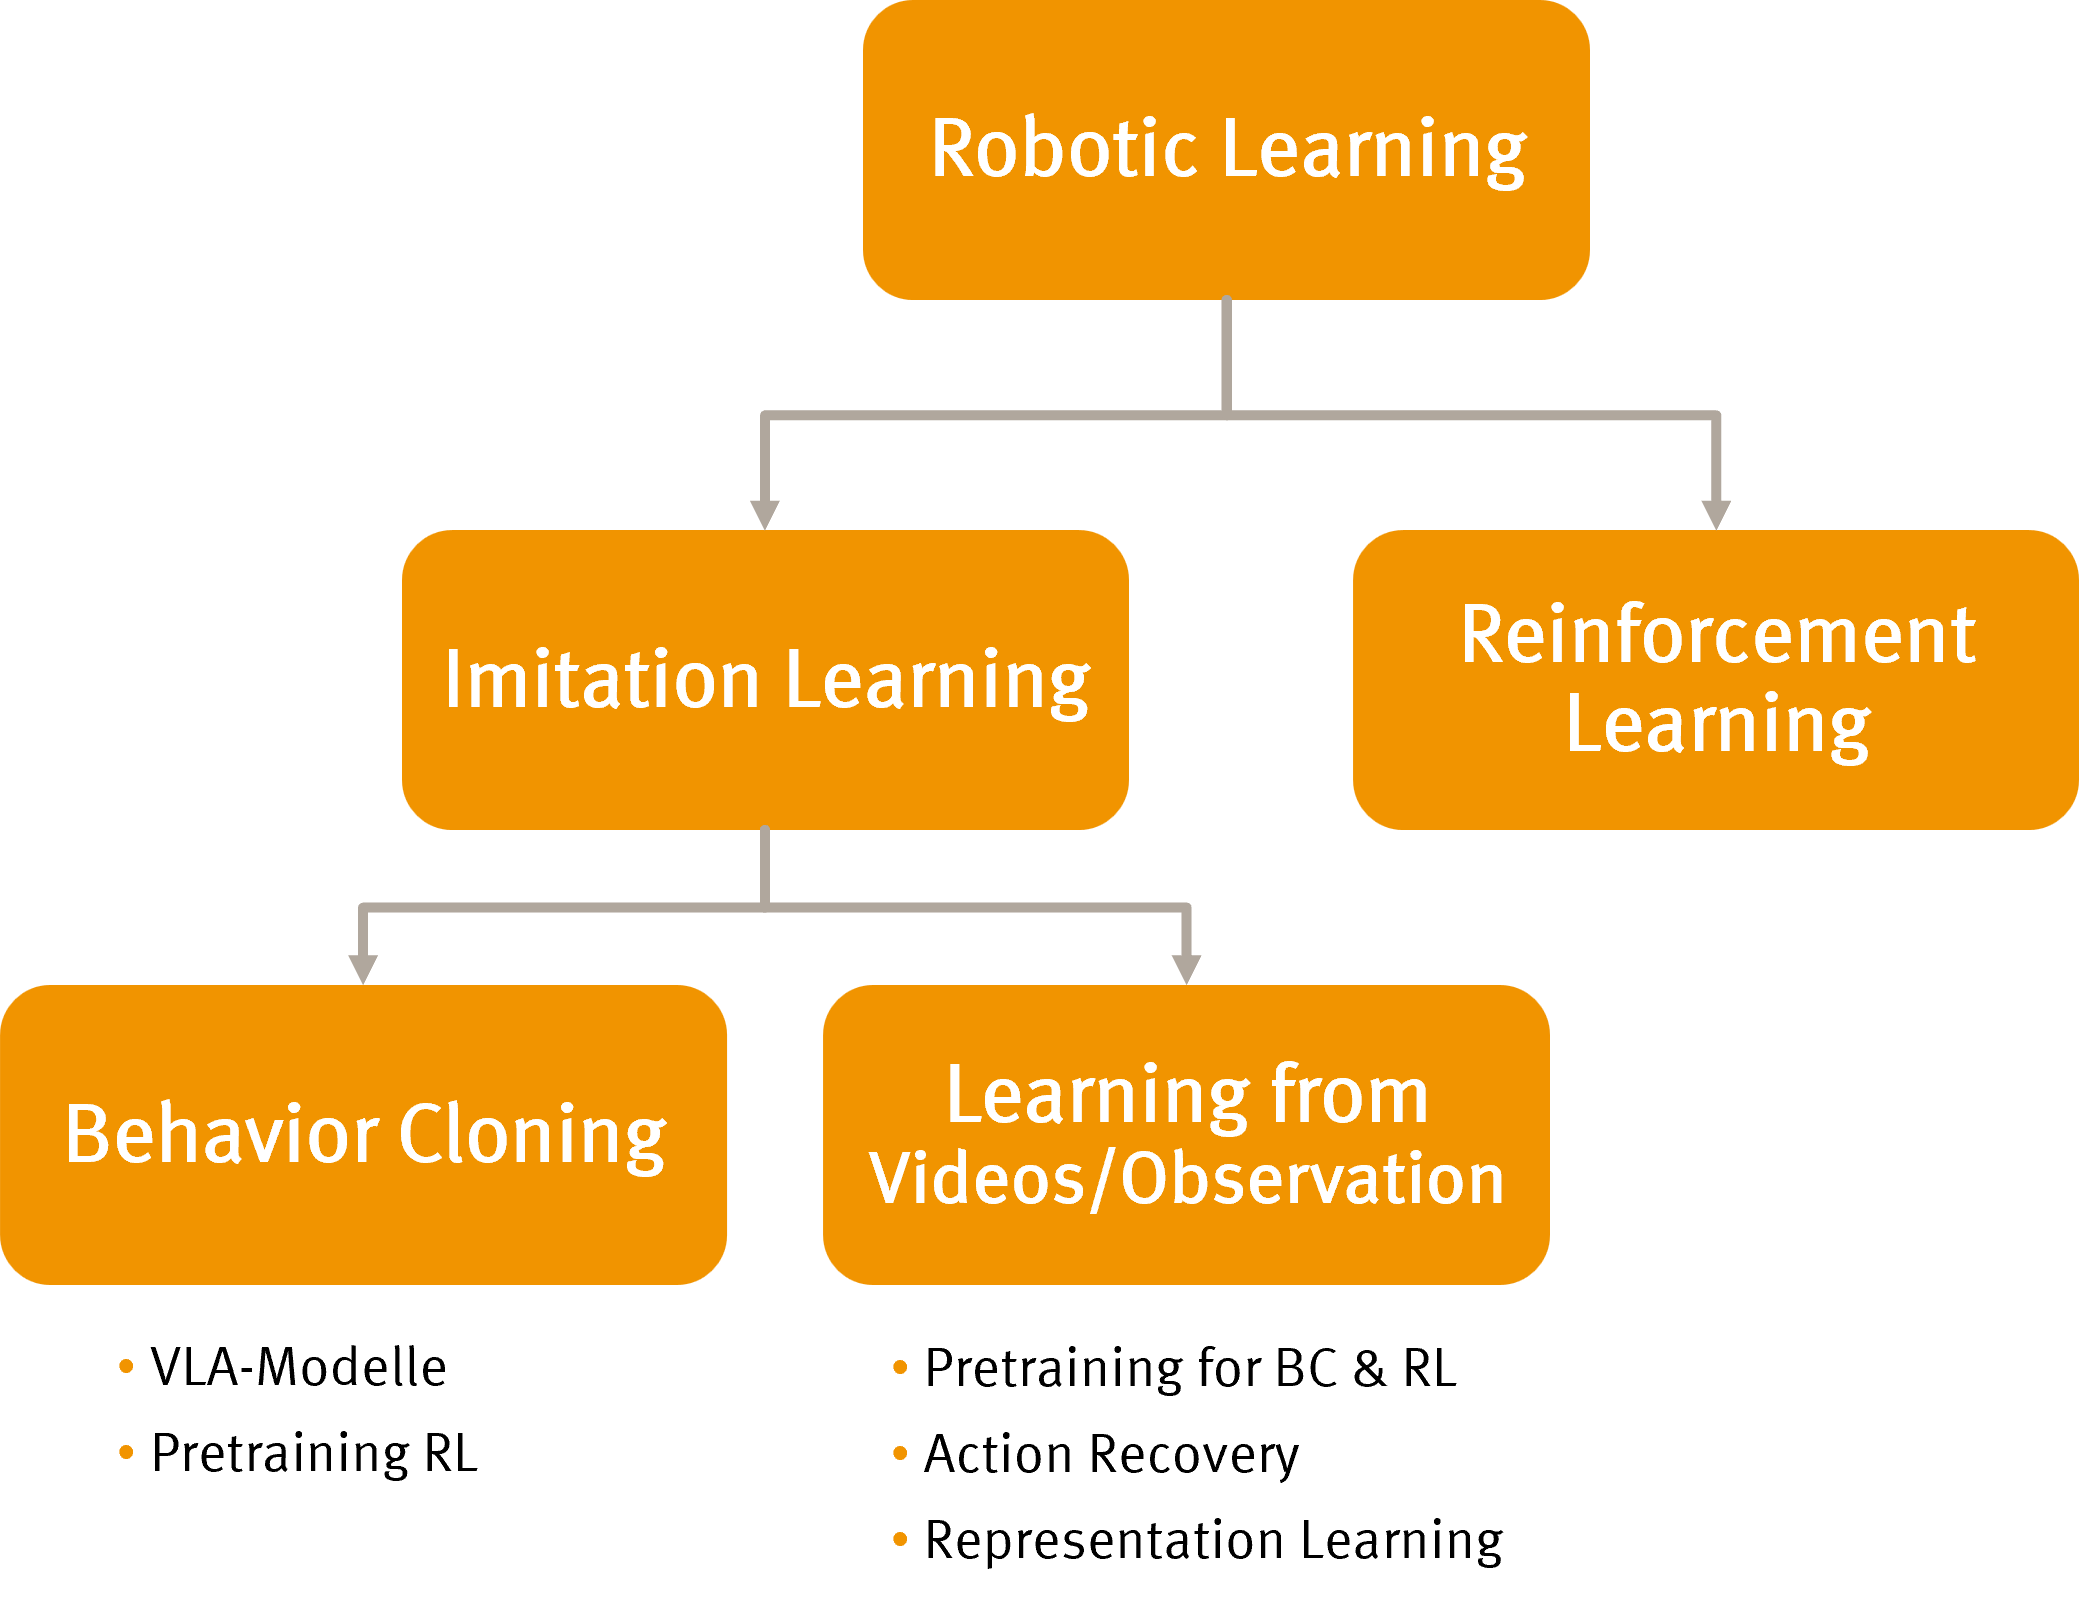
\includegraphics[width=0.6\linewidth]{./chapter3/media/OverviewRoboticLearning}
	\caption[Hybrid Approaches: Overview Robotic Learning]{Hybrid Approaches: Overview Robotic Learning}
	\label{fig:overviewroboticlearning}
\end{figure}

For example, methods from the \ac{LfV} paradigm can be used for action recovery, making unannotated video data applicable for \ac{BC} by recovering or estimating the underlying actions \cite{McCarthy_2025}. Furthermore, such methods can be employed to pretrain models for \ac{BC} or \ac{RL} by learning expressive state and action representations through representation learning \cite{McCarthy_2025}.

\ac{BC} is also widely used for training \ac{VLA} models and for pretraining \ac{RL} \ac{KM}s, for instance by learning components like value functions or reward models \cite{McCarthy_2025, Eze2024LearningBW}.


A common strategy is to use \ac{IL} for policy initialization, followed by RL-based fine-tuning to improve long-horizon performance and adapt policies through interaction with the environment \cite{Ramachandruni2020AttentiveTS, peng2018sfv}. Other approaches incorporate \textit{Residual RL}, where \ac{RL} refines or corrects imperfect demonstration trajectories, enabling adaptation to different robot embodiments or environmental conditions \cite{GarciaHernando2020PhysicsBasedDM}.
Hybrid methods are also widely used for \textit{domain adaptation}. By leveraging semantic priors, representation learning \cite{peng2018sfv, Ramachandruni2020AttentiveTS} or adversarial objectives \cite{GarciaHernando2020PhysicsBasedDM}, these approaches enable robots to transfer skills across different domains, viewpoints and embodiments, even when demonstrations are unaligned or originate from third-person videos \cite{Stadie2017ThirdPersonIL, Ramachandruni2020AttentiveTS, Pertsch2022CrossDomainTV, Aytar2018PlayingHE}.
More recent work further \textit{combines RL and IL with control-theoretic methods} such as \acf{MPC}, improving trajectory optimization, safety and real-world deployment robustness \cite{Huo2023EfficientRS}. \ac{MPC} is an advanced control strategy that uses a Dynamics Model $p(o_{t+1} \mid o_{t-k:t}, a_t),$ to predict future behavior \cite{Sacks2022LearningTO}.




% In practice, \ac{BC} and \ac{LfV} are often combined to exploit the advantages of both approaches, enabling the use of large-scale unannotated data while maintaining the efficiency of supervised policy learning.


\paragraph{Discover the Usage of Video Data for \acs{RL} Knowledge Modalities}

\ac{RL} can benefit from knowledge extracted from large-scale video data in multiple ways. In the following section, we analyze how information obtained from videos can be incorporated into different RL Knowledge Modalities in order to improve learning efficiency and overall performance:
\begin{itemize}
    \item Policy (Section \ref{sec:HybridPolicies})
    \item Dynamics Model (Section \ref{sec:DynamicsModels})
    \item Reward Functions (Section \ref{sec:RewardFunctions})
    \item Value Functions (Section \ref{sec:ValueFunctions})
\end{itemize}



\subsection{Policies}
\label{sec:HybridPolicies}
\begin{figure}[!ht]
	\centering
	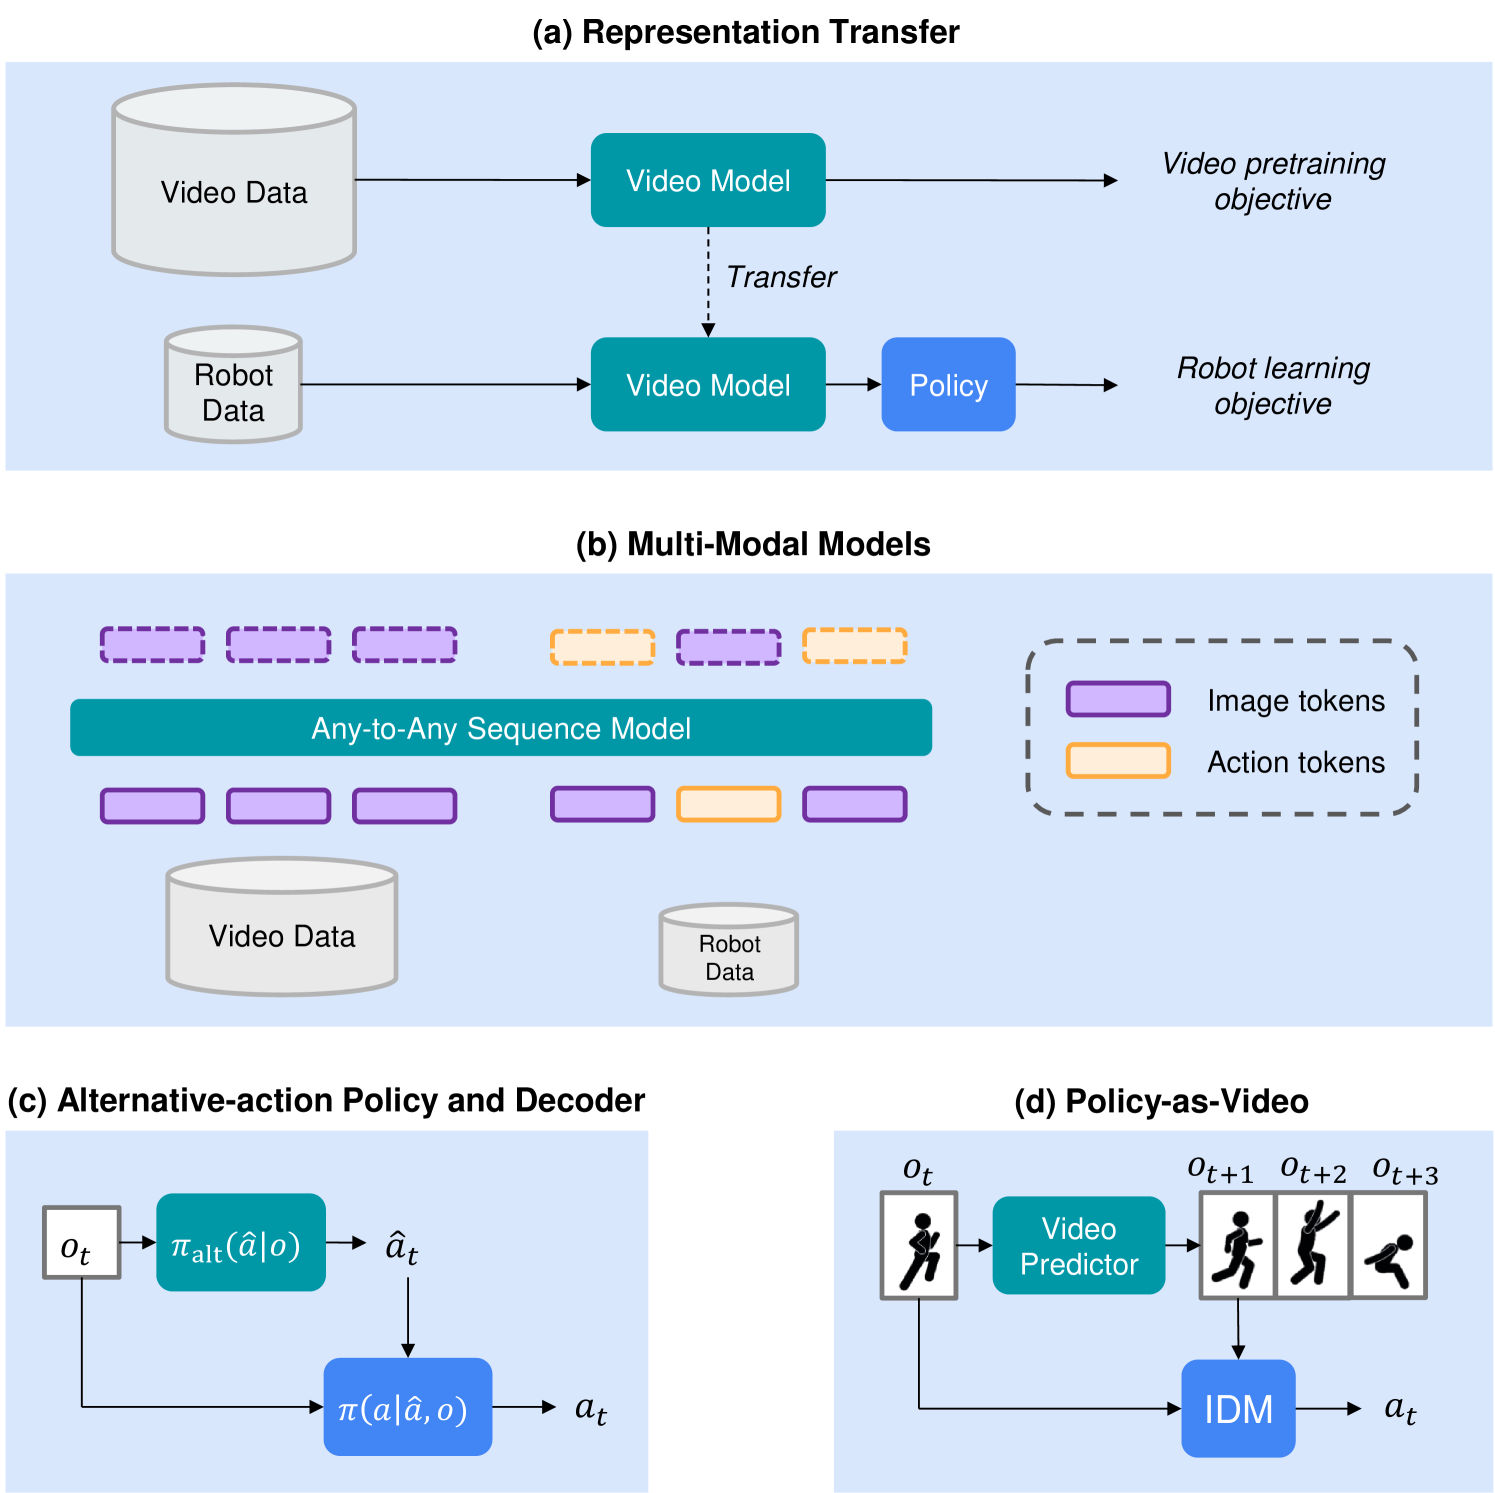
\includegraphics[width=1.0\linewidth]{./chapter6/media/LearningPoliciesFromVideo}
	\caption[Hybrid Approaches: Learning policies from video]{Hybrid Approaches: Learning policies from video. Image source: \cite{McCarthy_2025}.}
	\label{fig:LearningPoliciesFromVideo}
\end{figure}


% ToDo: what are with these texts?
% Representations can be pretrained from video data and used downstream whilst training a policy on robot data. 
% Jointly train on video, robot, image and text data to predict actions to predict robot actions. 
% A policy trained to output an action representation which conditions an action-decoding policy trained on robot data. 
% specific instantiation: hierarchical setup where the action representation is a video and the decoder is (often) an inverse dynamics model (IDM)


The core idea is to learn useful representations, actions, or abstractions from video data $D_{video}$ to improve the robot policie $\pi$ %(a_t \mid o_t)$ 
\cite{McCarthy_2025}.

\paragraph{a) Representation Transfer}
Large-scale video data can be leveraged to pretrain visual models that learn semantically meaningful representations of environments, objects and task dynamics. Instead of learning directly from limited robot interaction data, the agent first acquires general visual priors from diverse video datasets. These pretrained representations can subsequently be transferred to downstream policy learning, where they improve both data efficiency and generalization capabilities.

In this setting, Video Foundation Models (see Section~\ref{sec:ExtractingFoundationalKnowledgeFromInternetVideo}) are typically trained using self-supervised or unsupervised objectives on large collections of videos. The learned visual encoder captures high-level features such as object permanence, motion patterns, spatial relationships and temporal consistency. During downstream reinforcement or \ac{IL}, the pretrained encoder is either frozen or fine-tuned while the policy is optimized on robot-specific data \cite{McCarthy_2025}.

The main advantage of representation transfer is that the policy no longer needs to learn low-level visual features from scratch. Instead, it can focus on task-specific decision making, substantially reducing the amount of robot interaction required for effective learning. Furthermore, pretrained representations often generalize better across environments, viewpoints and object variations, making policies more robust in real-world settings.

Several large-scale studies have demonstrated the effectiveness of transferring representations learned from video data to robotic policy learning \cite{Jing2023ExploringVP, Silwal2023WhatDW, Zhao2022WhatMR, Burns2023WhatMP, Hu2023ForPV, Majumdar2023WhereAW}.


\paragraph{b) Multi-Modal Models}
Multi-modal models can be trained on a combination of videos, images, texts and robot specific data to learn shared representations that can predict robot actions, see \autoref{fig:LearningPoliciesFromVideo}, illustration (b). By jointly optimizing on diverse data sources, these models can leverage the rich contextual information from the different modalities while grounding their outputs in robot-compatible action spaces $A$ or $\hat{A}$ \cite{McCarthy_2025}. For more infos see \autoref{sec:MulitModalModelsExtractingFoundationalKnowledgeFromVideos} or \autoref{sec:MultiModalApproachesVLAModels}.

\paragraph{c) Alternative Action Policy $\pi_{\hat{A}}(\hat{a}_t|o_t)$ and Decoder $\pi(a_t|\hat{a}_t, o_t)$}
% \paragraph{d) Alternative-action Decoders $\pi(a_t|\hat{a}_t, o_t)$}
\underline{Alternative action Policy $\pi_{\hat{A}}(\hat{a}_t|o_t, c_t)$:}
\label{sec:AlternativeActionPolicy}

An alternative-action policy $\pi_{\hat{A}}(\hat{a}_t|o_t, c_t)$ learns to predict an alternative Action Representation $\hat{a}_t \in \hat{A}$ based on observation $o$ and some other conditional information $c$, rather than directly outputting low-level robot actions. For Further Information about alternative action representations see Section~\ref{sec:AddressingMissingActionLabelsAndDistributionShift}. 

alternative-action policies are typically trained on large-scale internet video data to gather diverse behavioral patterns and general knowledge about the world and physical interactions \cite{Schmidt2023LearningTA}.

A common training procedure assumes that the video data contains approximately expert behaviour. The videos are first labelled with alternative-action representations, after which the alternative-action policy $\pi_{\hat{A}}(\hat{a}_t \mid o_t, c_t)$ is trained using supervised behaviour cloning objectives \cite{Schmidt2023LearningTA,Bruce2024GenieGI,Wang2023MimicPlayLI,Du2023VideoLP,Black2023ZeroShotRM,Wen2023AnypointTM,Bharadhwaj2023TowardsGZ}. The learned policy can then either be used directly for representation transfer or to condition a downstream action decoder $\pi(a_t \mid \hat{a}_t, o_t)$ trained on robot interaction data.

When the behaviour contained in the video data is noisy or suboptimal, additional conditioning signals can improve learning. In particular, language conditioning \cite{Du2023VideoLP,Wen2023AnypointTM} and goal conditioning \cite{Wang2023MimicPlayLI} help constrain the learned behaviour towards task-relevant objectives. Offline \ac{RL} may provide another mechanism for leveraging imperfect demonstrations, although this direction remains relatively underexplored in the current literature \cite{McCarthy_2025}.

Several recent approaches instantiate alternative-action policies using pretrained \acp{VLM} or \acp{LLM} on internet-scale data. For example, \textcite{Yang2023LearningIR,Du2023VideoLP,Mu2023EmbodiedGPTVP} finetuned VLMs or LLMs to produce language-based action representations. In contrast, \textcite{Black2023ZeroShotRM} train an image-editing diffusion model that transforms the current observation into a predicted subgoal image, which serves as the alternative-action representation.




\underline{Alternative Action Decoder $\pi(a_t|\hat{a}_t, o_t)$:}
\label{sec:AlternativeActionDecoder}

A separate action decoder $\pi(a_t|\hat{a}_t, o_t)$ can subsequently be trained on robot data to map these alternative action representations $\hat{a}_t \in \hat{A}$ to real robot actions commands $a_t$. This approach employs an alternative action strategy and a decoder that effectively decouple the learning of high-level action representations from low-level control, allowing the policy to leverage rich information from video data while still grounding its outputs in robot-compatible actions \cite{Schmidt2023LearningTA, Du2023LearningUP, Wen2023AnypointTM}.
There exist two approaches to obtain the decoder:

\textit{Learning the decoder.}
In this setting, the robot dataset $D_{robot}$ is augmented with alternative action representations, resulting in tuples of the form $(o_t, \hat{a}_t, a_t, o_{t+1})$. The decoder $\pi(a_t \mid \hat{a}_t, o_t)$ can then be trained using supervised learning objectives to predict low-level robot actions conditioned on both the current observation and the alternative action representation \cite{McCarthy_2025, Schmidt2023LearningTA, Bruce2024GenieGI, Wang2023MimicPlayLI, Wen2023AnypointTM, Du2023LearningUP, Black2023ZeroShotRM}. 

Other Approaches to learn a decoder include:
\begin{itemize}
    \item Instead of keeping the alternative-action policy fixed, some approaches jointly optimize the compositional policy
    \begin{equation}
    \pi(a_t \mid \pi_{\hat{A}}(\hat{a}_t \mid o_t), o_t)
    \end{equation}
    using online \ac{RL}, enabling end-to-end training between high-level planning and low-level control \cite{Schmidt2023LearningTA}.
    \item \textcite{Jain2024Vid2RobotEV} learns a direct mapping from human demonstration videos to robot actions from paired human-video and robot-trajectory data in an end-to-end setting.
\end{itemize}


\textit{Manually defining the decoder.}
Instead of learning the decoder from data, the decoder can be manually crafted using explicit engineered geometric or kinematic mappings. 
Manually defined decoders reduce the need for paired robot supervision and can incorporate strong inductive biases about the robot embodiment. 
%  These methods exploit engineered correspondences between visual motion cues and robot control commands.
Examples of manually defined decoders include:
\begin{itemize}
    \item Inferring low-level robot actions from optical flow patterns in the video, which capture the direction and magnitude of motion in the scene \cite{Ko2023LearningTA, Yuan2024GeneralFA}.
    \item Mapping robot actions to visual arrows, which projecting future robot pose as on-screen hints and subsequently decoding them back into executable control commands \cite{Nasiriany2024PIVOTIV}.
    \item Retargeting human hand poses or body motions to equivalent robot joint commands \cite{Qin2021DexMVIL, Sivakumar2022RoboticTL}.
\end{itemize}
% However, they often require task-specific engineering and may generalize less effectively across diverse environments and robot platforms compared to learned decoding approaches.



\underline{Example Workflow: Policy-as-Video}

In this workflow, generated videos serve directly as the policy output. The alternative action Space $\hat{A}$ refers to the paradigm \textit{observation-as-action}, see \autoref{sec:CategoriesOfAlternativeActionRepresentations} illustration (d). The procedure consists of two steps \cite{Du2023LearningUP, McCarthy_2025} accouring to Figure~\ref{fig:LearningPoliciesFromVideo} illustration (d):
\begin{enumerate}
    \item A \textbf{language-conditioned video predictor} $p(\tau \mid o_{t-k:t}, c)$, generates a future video sequence that imagines successful task completion given the current observation and a language instruction as context. $\tau$ represents a generated video trajectory and $c$ the conditional informations.
    
    \item An \textbf{action-decoding \acf{IDM}} $p^{-1}(a_t \mid o_t, o_{t+1})$ is used to infer low-level robot actions $a_t$ from these generated video frames. The IDM is trained on the robot dataset $D_{\text{robot}}$.
\end{enumerate}


Potential improvements of this compositional approach include:
\begin{itemize}
    \item Compositional alignment between video, language and the IDM actions within a multi-modal approach, where each modality informs the others \cite{Ajay2023CompositionalFM}.
    \item Improving the action decoding model by incorporating goal-conditioned behavior cloning \cite{Du2023VideoLP}.
    \item Add additional conditioning modalities of alternative action representations $\hat{A}$ to the \ac{IDM} to improve the predicted low-level robot actions.
\end{itemize}



% ToDo: Disussion Section of the RL Policy Modality
\paragraph{Summary \& Limitations}
Overall, hybrid approaches provide a flexible framework that combines the strengths of multiple learning paradigms.
This synergy enables robots to learn more robust skills \cite{Radosavovic2022RealWorldRL, Nair2022R3MAU, Parisi2022TheUE} from limited demonstrations \cite{Nair2022R3MAU, Schmidt2023LearningTA, Ye2023ReinforcementLW} and generalize more effectively across tasks and environments \cite{Du2023LearningUP, Wang2023MimicPlayLI, Black2023ZeroShotRM, Thomas2023PLEXMT, Zhao2022WhatMR, Lin2023SpawnNetLG}.
% adapt policies online, --> no source

One question that has not yet been clarified is whether $\hat{A}$ is best suited for use in a hierarchical setup or offers greater value in representation transfer \cite{McCarthy_2025}. Furthermore, it must in hierachical approaches $\pi(a_t \mid \pi_{\hat{A}}(\hat{a}_t \mid o_t), o_t )$ be investigated to what extent the performance gap lies on $\pi$ or $\pi_{\hat{A}}$ \cite{McCarthy_2025}.





\subsection{Dynamics Models}
\label{sec:DynamicsModels}
Dynamic models $p(o_{t+1}|o_t, a_t)$ aim to determine how the environment evolves over time by predicting future observations based on the current state and the next action to be taken.
To learn dynamics models from video data, the core idea is to leverage the rich temporal and physical information contained in videos to train models that can capture the underlying dynamics of the environment \cite{McCarthy_2025}.


One common approach is to first pretrain a video prediction model $p(o_{t+1} \mid o_t)$ on large-scale video datasets $D_{video}$ in order to learn general temporal dynamics and physical interactions of the environment \cite{Yang2023LearningIR, Du2023LearningUP, Du2023VideoLP}. The pretrained model is subsequently adapted into a robot dynamics model $p(o_{t+1} \mid o_t, a_t)$ using robot interaction data $D_{robot}$, incorporating the influence of robot actions on future environment states \cite{McCarthy_2025}. This transfer enables the model to leverage broad visual world knowledge learned from internet videos while grounding the predictions in robot-specific control dynamics.

Another approach is the usage of alternative action representations by training an alternative-action video predictor $p_{\hat{A}}(o_{t+1} \mid o_t, \hat{a}_t)$, where $\hat{a}_t$ denotes high-level actions or latent behavioural representations extracted from video data \cite{Bruce2024GenieGI, Yang2023LearningIR, Du2023VideoLP, Du2023LearningUP, Rybkin2018LearningWY, Mendonca2023StructuredWM, Yuan2021DMotionRV, Wang2023ManipulateBS}. The learned alternative-action representations can subsequently condition a downstream action decoder trained on robot data. Conditioning on an alternative action space $\hat{A}$ provides greater control over generated trajectories and often enables mappings between abstract video-derived actions and executable robot actions \cite{Rybkin2018LearningWY, Schmidt2023LearningTA}.
\ac{LfV} video predictors have been conditioned on:
\begin{itemize}
    \item Language-as-actions \cite{Yang2023LearningIR, Du2023VideoLP}
    \item Single-step latent actions \cite{Rybkin2018LearningWY, Bruce2024GenieGI}
    \item Goal images \cite{Du2023LearningUP}
    \item Future grasp-location and post-grasp waypoint affordance information \cite{Mendonca2023StructuredWM}
    \item Motion information \cite{Yuan2021DMotionRV, Wang2023ManipulateBS}
    \item Multiple modalities \cite{Yang2023LearningIR}
    % \item [306] condition on several different action-spaces, including robot actions, language actions and camera motions
\end{itemize}

A further direction jointly pretrains dynamics models on both video $D_{video}$ and robot datasets $D_{robot}$ \cite{Yang2023LearningIR}. Recent approaches such as UniSim \cite{Yang2023LearningIR} extend this paradigm by conditioning dynamics models on actions across multiple modalities, including robot motor commands, language instructions, actions extracted from camera motions and other video-derived action representations.
% ToDo: i dont know if "other video-derived action representations" correct, but i think




\paragraph{Adaptation of video predictors to robot dynamics models}
Adaptation of video predictors to robot dynamics models often involves a fine-tuning step using robot interaction data $D_{robot}$ \cite{Du2023LearningUP, Ajay2023CompositionalFM}.
One challange is that naive finetuning on robot data result in the erasure of %pretraining 
knowledge acquired during large-scale video pretraining. To mitigate this issue, \cite{Seo2022ReinforcementLW} preserve pretrained knowledge by stacking an action-conditioned prediction model on top of the pretrained video predictor instead of directly modifying the entire model. 
\textcite{Mendonca2023StructuredWM} first applies video-based conditioning mechanisms during pre-training and subsequently incorporates robot-specific action conditioning in the adaptation phase. 
\textcite{Yang2023ProbabilisticAO} demonstrate that the score function of a large pretrained video diffusion model can guide the generation process of a smaller task-specific video model, enabling efficient specialization while retaining knowledge from large-scale pretraining.
Adaptation can furthermore involve learning mappings from alternative action representations $\hat{A}$ to executable robot actions \cite{Rybkin2018LearningWY}.

The resulting dynamics models can then be used for 
\begin{itemize}
    \item \textbf{Generate synthetic training data:}
    The model can generate synthetic training data by simulating how the environment evolves in response to different actions \cite{Yang2023LearningIR, Bruce2024GenieGI}. This allows for data augmentation and policy training without requiring real-world robot interaction. 
    \item \textbf{Differentiable Simulator:}
    By enabling backpropagation through model-generated rollouts, the dynamics model allows policies to be trained end-to-end using gradient-based optimization \cite{Seo2022ReinforcementLW, Wu2023PretrainingCW, Hafner2023MasteringDD}. This is especially useful for learning complex behaviors efficiently.
    \item \textbf{Planning and Control:}
    The dynamics model can be used for model-based control and trajectory planning, allowing the robot to anticipate the consequences of its actions and make informed decisions. Examples are here tree search \cite{Du2023VideoLP} and \acf{MPC} \cite{Rybkin2018LearningWY, Mendonca2023StructuredWM}. \ac{MPC} optimizes a trajectory over a short horizon and replans frequently. Tree search systematically simulates and evaluates many possible action sequences, often over a longer or variable horizon, by branching at each decision point. %This allows it to consider more possibilities and deeper future outcomes than MPC.
    % ToDo: Tree Seach and MPC explaination
    % Model Predictive Control (MPC):
    % MPC uses the model to predict a sequence of future states over a fixed planning horizon. At each step, it optimizes a sequence of actions, but only executes the first action before re-planning at the next step. This approach is typically continuous and re-optimizes as new observations come in.

    % Tree Search:
    % Tree search explores many possible sequences of actions by branching at each decision point, simulating different action paths (like building a tree of possibilities). It evaluates these branches to find the most promising sequence, which can be more exhaustive but is often used for discrete or combinatorial problems.
    % ToDo: Sources?
    \item A dynamics models can be used as part of a larger policy learning framework, where the dynamics model provides a predictive component that informs policy updates, value estimation, or hierarchical decision making.
\end{itemize}

\paragraph{Evaluation of Model-Generated Trajectories}
To assess the quality of simulated trajectories, it is necessary to evaluate them using a value or reward function \cite{Seo2022ReinforcementLW}. The reward function can be learned from reward-labeled robot data or even from video data \cite{Mendonca2023StructuredWM, Rybkin2018LearningWY, Yang2023LearningIR, Du2023VideoLP}. This enables the model to assign meaningful scores to predicted outcomes and guide decision-making.


\paragraph{Discussion}

% ToDo: ist ja eigl. vom original paper --> Quelle erwähnen?
Large pretrained video foundation models demonstrate strong generalization capabilities and enable dynamics models to learn useful world knowledge even from non-expert internet video data \cite{Yu2020MOPOMO}. In particular, diffusion-based video models have shown promising performance for long-horizon prediction and planning tasks \cite{Du2023VideoLP, Yang2023LearningIR}.

Future research directions include scalable alternative action $\hat{A}$ conditioning methods \cite{Bruce2024GenieGI} or hierarchical world models that combine video-level abstractions with robot-level control \cite{LeCun2022APT}. % and integrating learned video predictors \cite{Yang2023LearningIR} with classical physics simulators \cite{Gao2026NVIDIAIS}. 
% Another promising avenue is the generation of synthetic robot training data and trajectory rollouts using large pretrained video generation models \cite{Yang2023LearningIR, Bruce2024GenieGI} or enhance existing dataset diversity through video editing techniques \cite{Yu2023ScalingRL}. 
An underexplored direction is to combine standard analytic or physical simulation \cite{Gao2026NVIDIAIS} with video prediction simulation systems \cite{Yang2023LearningIR} to combine the physical accuracy and controllability of analytic simulators with the strong visual realism and planning capabilities of video predictors. Another promising avenue is the generation of synthetic robot data for training data, the generation of trajectory rollouts using large pretrained video generation models \cite{Yang2023LearningIR, Bruce2024GenieGI} or to enhance existing dataset diversity through video editing techniques \cite{Yu2023ScalingRL}. 

% Inspired by synthetic data practices in other domains \cite{Wang2024HelpSteer2OD, numina_math_7b}, future research could leverage foundational video predictors to create synthetic video rollouts \cite{Yang2023LearningIR, Bruce2024GenieGI} or to expand and enhance existing dataset diversity through video editing techniques \cite{Yu2023ScalingRL}.

Overall, video-based dynamics models provide a scalable framework for bridging visual world understanding and robot control through large-scale video pretraining, action conditioning and model-based planning.

% model-based control, trajectory planning, or as part of a larger policy learning framework.


% > Pretraining on massive video data, adding action conditioning and using models for simulation or planning are key to scalable robot learning.




\subsection{Reward Functions}
\label{sec:RewardFunctions}

Reward functions are a central component of \ac{RL}, as they define the objective that guides policy optimization. However, manually designing reward functions for open, complex and unstructured robotic environments is difficult, often task-specific and hard to scale \cite{McCarthy_2025}. To address this limitation, \ac{LfV} approaches aim to automatically extract visual reward functions directly from video data. The core idea is to transform robot transition tuples $(o_t, a_t, o_{t+1})$ into reward-annotated tuples $(o_t, a_t, r_t, o_{t+1})$, enabling their use in both online and offline \ac{RL} settings \cite{McCarthy_2025}.


\underline{Video-Language Model as Reward Functions}


One common approach is to use Video-Language Models (VidLMs) to derive reward signals from language descriptions and video observations. \textcite{McCarthy_2025} identify two categories of methods:
\begin{itemize}
    \item \textbf{Video-text similarity:} Dual-encoder architectures embed videos and natural language instructions into a shared representation space \cite{Xu2021VideoCLIPCP, Zhao2024VideoPrismAF}. The reward is defined as the similarity between the robot observation and the language-conditioned task representation in the embedding space \cite{Sontakke2023RoboCLIPOD, Fan2022MineDojoBO, Ding2023ReinforcementLF}.
    
    \item \textbf{\acf{VQA}:} Video-to-text models (see Section~\ref{sec:VideoToTextModels}) answer questions about the current state of the task, such as whether the task has been completed or estimating the current task progress. The answers could then used to provide dense reward signals that guide policy learning \cite{McCarthy_2025}. \cite{Du2023VideoLP, Yang2023RobotFM} used \ac{VQA} with images as input to provide rewards.
\end{itemize}



\underline{Video Prediction Models as Reward Functions}

Video prediction models $p(o_{t+1}|o_t)$ learn to predict future observations based on the current visual state of the environment.
% learn to predict the next frame from the current one. 
Such models can be converted into reward functions by measuring how likely the next performed robot action, as observed by it's camera, is under the pretrained video predictor \cite{Huang2023DiffusionRL, Zhu2023GuidingOR, Escontrela2023VideoPM}.
% Such models can be converted into reward functions by evaluating how likely the observed robot trajectory is under the pretrained video predictor.
% Such a model can be converted into a reward function by measuring how likely the action performed by the robot, observed by the robot's camera, occurs according to the model. 
In this setting, the robot receives a high reward when the actual next frame from the robot's camera closely matches the predicted future observations of the model. % model's prediction
This encourages the robot to produce behaviors whose visual dynamics resemble those observed in the video data used during pretraining. To improve scalability across diverse and non-expert internet videos, recent approaches \cite{Escontrela2023VideoPM} additionally condition the video predictor on language instructions, enabling task-specific reward generation for a broad range of behaviors.
% This encourages the robot to produce behaviors whose visual dynamics are similar to those in the video data the model was trained on. To scale this approach to diverse, non-expert internet videos, the video predictor can be conditioned on language instructions, allowing the reward to be tailored to various tasks.



\underline{Visual Feature Representational Similarity to a Reference as Reward Functions}

This approaches define the reward as the similarity between the current robot observation and a reference observation, such as goal images \cite{Ma2022VIPTU} or demonstration videos. In this setting, deep visual representations are used to compare the semantic similarity between observations rather than relying on raw pixel comparisons.

\textcite{Ma2022VIPTU} employ time-contrastive learning objectives, which provide implicit estimates of the temporal distance between two observations and therefore encode task progress information about the current robot observation and the visual reference. Meaningful visual representations are needed to address the distribution shift between human demonstrations and robot observations, like:
\begin{itemize}
    \item Viewpoint-invariant representations \cite{Aytar2018PlayingHE, Sermanet2017TimeContrastiveNS}
    \item Embodiment-invariant representations \cite{Zakka2021XIRLCI} %and teqchniqes to mitigate embodiment differences \cite{Qin2021DexMVIL, Mandikal2022DexVIPLD}
    \item Object-centric representations \cite{Sieb2019GraphStructuredVI, Kumar2022GraphIR, Chang2020SemanticVN}
\end{itemize}
Other methods \cite{Qin2021DexMVIL, Mandikal2022DexVIPLD} apply pose retargeting techniques to map human motions to robot-compatible embodiments before computing the reward signal.
% ToDo: maby refernce to representation learning and domain adaption
% Pose retargeting techniques additionally enable comparisons across different embodiments by mapping human motions to robot-compatible representations.






% \underline{Potential-based Shaping with Value Functions}
% Dense reward signals can be obtained from pretrained value functions $V(o_t)$ or $Q(o_t, a_t)$. A value function estimates the future task progress or success likelihood based on the current observation and is learned from video demonstrations using temporal-difference learning or time-contrastive objectives.

% The reward is then computed through potential-based reward shaping:
% \begin{equation}
% r_t = V(o_{t+1}) - V(o_t)
% \end{equation}
% This formulation provides smooth and dense optimization signals, which can significantly improve the stability and efficiency of downstream \ac{RL}.

\underline{Tracking Objects and Interactions}

Some approaches \cite{Chang2020SemanticVN} leverage object labels together with off-the-shelf object detectors to infer task progress and goal states from observations. In manipulation tasks, object detectors can identify relevant objects, locations or the robot gripper in each frame. By tracking these objects over time, the system can estimate task progress and automatically derive reward signals. For example, decreasing distance between the gripper and an object may indicate approach behavior, while object movement together with gripper interaction can signal successful grasping or task completion. This enables the generation of goal and reward annotations without requiring manually labeled demonstrations.

\underline{Potential-based Shaping with Value Functions}

% ToDo: The context c is correct i think. It was is the paper 'TOWARDS UNIVERSAL VISUAL REWARD AND REPRESENTATION VIA VALUE-IMPLICIT PRE-TRAINING'
Dense reward signals can be obtained from pretrained value functions $V(o_t)$ or $Q(o_t, a_t)$, where $c$ represents the goal condition of the task. The value function estimates how much progress has been made toward achieving the goal represented by $c$ from the current observation $o_t$ \cite{2022TowardsUV}.
% Dense reward signals can be obtained from pretrained value functions $V(o_t)$ or $Q(o_t, a_t)$. The value function estimates how much progress has been made toward achieving the goal based on the reward function from the current observation $o_t$.
% A value function estimates the expected future task progress or the likelihood of eventual success from a given observation. 
Such value functions can be learned from video demonstrations using either Temporal-Difference (TD) learning \cite{Chang2022LearningVF} or Time-Contrastive learning \cite{Ma2022VIPTU}, see Section~\ref{sec:ValueFunctions}.

Once a value function $V(o_t, c)$ is learned, it can be used to generate a dense reward signal via potential-based reward shaping \cite{McCarthy_2025}:
\begin{equation}
r_t = V(o_{t+1}, c) - V(o_t, c)
\end{equation}
This reward is positive when the robot moves toward states with higher predicted success (i.e. makes progress toward the goal) and negative when it regresses. This formulation provides smooth and dense optimization signals, which can significantly improve the stability and efficiency of downstream \ac{RL}.
The principle can be applied to action-value functions $Q(o_t, a_t, c)$ too.
% I dont know if it is right, we need there a paper!, where the reward is defined as the difference in predicted value before and after taking an action.





\underline{\acf{GAIL}}

\ac{GAIL} trains a policy and a discriminator simultaneously in an adversarial game \cite{Ho2016GenerativeAI, Torabi2018GenerativeAI}.
\begin{itemize}
    \item The \textbf{discriminator} is trained to distinguish between state-action pairs coming from expert demonstrations (e.g. vidoes) and those generated by the current robot policy.
    \item The \textbf{robot policy} is trained to produce state-action pairs that fool the discriminator into thinking they came from the expert.
\end{itemize}
In this setup, the discriminator's output serves as a \textbf{learned reward signal}: When the robot's behavior looks similar to the expert, the discriminator is uncertain and gives a high score. When the behavior looks different, the discriminator confidently classifies it as fake and gives a low score \cite{Torabi2018GenerativeAI}. 
% The robot policy is then optimized (using standard RL) to maximize this score. 
The result is that the robot learns to maximize this score and match the distribution of behaviors observed in the video demonstrations, without ever receiving an explicit reward function.

% Generative Adversarial Imitation Learning (GAIL) approaches aim to match the behavior distribution observed in video demonstrations during online \ac{RL}. In this setting, the robot policy is optimized such that the produced trajectories from the robot policy become indistinguishable from trajectories coming from expert demonstrations, contained in the video dataset.
% \begin{itemize}
%     \item The \textbf{discriminator} is trained to distinguish between state-action pairs coming from the expert demonstrations (e.g., videos) and those generated by the current robot policy.
%     \item The \textbf{robot policy} is trained to produce state-action pairs that fool the discriminator into thinking they came from the expert.
% \end{itemize}

Since human demonstrations and robot observations often differ significantly in viewpoint, embodiment and visual appearance, these approaches typically require invariant feature representations to reduce the impact of distribution shift between video and robot domains \cite{Qin2021DexMVIL, Stadie2017ThirdPersonIL}.
% These approaches often require invariant feature representations to handle distribution shifts between human demonstrations and robot observations.



\underline{Other Reward Extraction Methods}

Additional methods train a task classifier on task-labelled video datasets to provide downstream reward signals for \ac{RL} \cite{Chen2021LearningGR, Shao2020Concept2RobotLM}. 
Other approaches estimate the number of remaining steps-to-completion in a video and use this quantity as a proxy signal for task progress \cite{Edwards2019PerceptualVF, Yang2023LearningIR}.

Further work encourages similarity to video-derived behavioral priors, such as pretrained video policies \cite{Ye2023ReinforcementLW} or human affordance distributions \cite{Bahl2023AffordancesFH}, allowing the robot to align its behavior with patterns extracted from large-scale video demonstrations.


\paragraph{Downstream Usage of LfV Reward Functions}

Video-pretrained reward functions can either be transferred zero-shot to downstream robotic tasks \cite{Escontrela2023VideoPM} or further finetuned on robot data $D_{robot}$ \cite{Sontakke2023RoboCLIPOD}. The extracted rewards may serve as the sole optimization objective for \ac{RL} \cite{McCarthy_2025}, or act as auxiliary shaping and exploration rewards in combination with sparse rewards \cite{Zhen20243DVLAA3, Chang2022LearningVF}. In some approaches \cite{Adeniji2023LanguageRM}, the reward functions are additionally used to pretrain policies before subsequent finetuning the reward model on manually defined task rewards.


\paragraph{Summary}

Compared to directly learning policies or dynamics models, reward functions are often easier to extract from large-scale video data, since they only require estimating task progress or behavioral similarity rather than generating complete action sequences \cite{McCarthy_2025}. 
% ToDo: source
Recent advances in pretrained foundation models, particularly video-language models and video prediction architectures, have significantly improved the quality and scalability of visual reward extraction.

Future research directions include combining \ac{LfV} reward functions with other video-based \acp{KM} or finetuning policies through online \ac{RL} using the learned reward functions \cite{Hafner2023MasteringDD, JyothirS2023GradientbasedPW}, as well as using \ac{LfV} rewards to augment reward annotations in datasets. Another promising avenue is the use of video-derived rewards for safety monitoring and constraint estimation \cite{Guan2024TaskSI}. Furthermore, extracting dense reward signals from video-to-text models through \acf{RL-AI-F} represents an emerging direction \cite{Klissarov2023MotifIM}.

Overall, video-based reward functions provide a scalable mechanism for translating visual demonstrations into optimization signals for \ac{RL}, reducing the need for manually engineered reward design in robotic systems \cite{McCarthy_2025}.









\subsection{Value Functions}
\label{sec:ValueFunctions}


Value functions play a central role in \ac{RL}, as they estimate the expected return or task progress from a given state or state-action pair \cite{Schulman2017ProximalPO, Haarnoja2018SoftAA}. In the context of \ac{LfV}, recent approaches investigate how value-function-like models can be pretrained on large-scale video data, with the goal of capturing task-relevant progress signals that can be transferred to downstream robotic control. State-action-value functions $Q(o_t, a_t)$ are preferable to state-value functions $V(o_t)$, because they offer more informative guidance for action selection and policy improvement \cite{sutton2018reinforcement}.


\paragraph{Pretraining: Temporal-Difference Learning}
One common approach is to pretrain value functions using the \ac{TD} learning \cite{sutton2018reinforcement}. \ac{TD} learning requires often access to actions, rewards and goal annotations, which are typically not available in raw video data. 
% LfV methods therefore introduce alternative formulations to address these missing supervision signals.

To handle missing action labels, state-value functions for example are often conditioned on alternative action representations $\hat{A}$, resulting in models of the form $V(o_t, \hat{a}_t)$ \cite{McCarthy_2025}. 

To adress the lack of reward and goal annotations, \ac{LfV} reward methods described in the Section~\ref{sec:RewardFunctions} can be used. Furthermore, video-to-text models can provide semantic goal descriptions in natural language, enabling value functions to be conditioned directly on textual task objectives \cite{McCarthy_2025}.

% Some approaches leverage object labels together with off-the-shelf object detectors to infer task progress and goal states from video. Consider a pick-and-place task where the robot must grasp a red cube and place it into a blue bin. An object detector pre-trained on common objects can identify the red cube, the blue bin and the robot’s gripper in each video frame. By tracking these objects over time, the system automatically determines progress: the distance between gripper and cube decreasing indicates approach; gripper closing with the cube moving signals a successful grasp; the cube entering the bin indicates task completion. No manual reward or goal labeling is required—only a set of relevant object labels and a standard detector.



\paragraph{Pretraining: Time-Contrastive Learning}

Value functions can be learned through time-contrastive learning \cite{Ma2022VIPTU}. 
% These methods enforce temporal consistency in the learned representation space such that observations closer to task completion are embedded closer to the goal state. A value function can then be defined as a distance measure between the current observation and a goal representation.
Time-contrastive Learning approaches learn task progress directly from the temporal structure of videos. The model is trained such that observations temporally closer to the goal condition $c$ obtain more similar representations, while temporally distant observations are separated in the embedding space. For example, a task can be specified via a set of goal images. The model learns that observations close in time to the goal should have high value, while observations far from the goal (in time) should have low value \cite{Ma2022VIPTU}. As a result, the learned representation implicitly captures progression toward task completion and can be used to derive dense reward signals from raw video demonstrations.

Other Approaches discover the use of:
\begin{itemize}
    \item \textbf{Quasimetric Functions:} Learn an asymmetric distance measurement that better captures task progress. For example, going from ``object on table'' to ``object in box'' is meaningful progress, while the reverse transition should not necessarily have the same distance \cite{Wang2023OptimalGR}.
    
    \item \textbf{Temporal cycle-consistency objectives:} Enforce that temporal correspondences between frames remain consistent across videos. If frame A in one video corresponds to frame B in another demonstration, the mapping should also hold when traced back, producing temporally aligned representations across demonstrations \cite{Zakka2021XIRLCI}.
\end{itemize}

These approaches do not require action labels, making them particularly suitable for large-scale video pretraining. However, they typically require explicit goal images or reference observations at training and inference time \cite{McCarthy_2025}. 


\paragraph{Pretraining: Heuristic and Weak Supervision}

Another line of work constructs value functions using heuristic supervision signals extracted from video data \cite{Edwards2019PerceptualVF}. A common strategy is to regress the number of remaining timesteps until task completion, effectively learning a time-to-go metric under the assumption of expert behavior in the provided task demonstration. Other approaches finetune vision-language models to predict such heuristic progress signals \cite{Du2023VideoLP}.

Some methods additionally identify key states in demonstration videos and use them to improve value estimation, although these approaches often still rely on some form of reward or success annotation in the training data \cite{Liu2023LearningTI}.




\paragraph{Downstream Usage}

Video-pretrained value functions can be used in several ways in downstream robotic learning. If the value function is explicitly action-conditioned $V(o_t, a_t)$ \cite{Chang2020SemanticVN} or alternative-action conditioned $V(o_t, \hat{a}_t)$ with a mapping to robot actions, it can be directly integrated into standard value-based \ac{RL} or planning frameworks \cite{Chang2022LearningVF}. When combined with a learned or given dynamics model $p(o_{t+1} \mid o_t, a_t)$, unconditioned value functions $V(o_t)$ can also be used for tree-search based planning \cite{Du2023VideoLP}.

In addition, pretrained value functions can serve as initialization for downstream policy or value networks, improving training efficiency in robot domains \cite{Bhateja2023RoboticOR}. They are also commonly used for potential-based reward shaping, where dense rewards are defined as $r_t = V(o_{t+1}) - V(o_t)$ to guide exploration in sparse-reward settings \cite{Edwards2019PerceptualVF, Ye2023ReinforcementLW, Chang2022LearningVF}. 
% ToDo: what is with this paragraph
Finally, value functions can accelerate \ac{TD} learning in downstream tasks by serving as bootstrap targets in Bellman updates \cite{Edwards2019PerceptualVF}.


\paragraph{Summary}
Research on learning value functions directly from videos remains relatively scarce, mainly due to missing action, reward and goal labels, as well as the multi-modal nature of human behavior in video data \cite{McCarthy_2025}. \ac{TD} learning from video shares similar challenges with offline \ac{RL} \cite{Levine2020OfflineRL}, but existing solutions from the literature (e.g. conservative regularization \cite{Kumar2020ConservativeQF} or latent action inference \cite{Zhou2020PLASLA}) offer potential fixes. Despite these difficulties, \ac{TD} learning of value functions from large-scale human video is increasingly seen as a promising direction for real-world robotics, enabling reward-free progress estimation and goal-conditioned policy learning \cite{Bhateja2023RoboticOR}.

% This formulation enables learning state-action value estimates from video even when true robot actions are unavailable.

% \begin{itemize}
%     \item \textbf{Temporal-Difference (TD) Learning} 
%     TD learning requires reward annotations, such as success or failure labels for the demonstration videos. The Value function is trained by comparing its current prediction $V(o_t, c)$ with the received reward $r_t$ plus the predicted future value $V(o_{t+1}, c)$ at the next step. The difference between these two quantities (the TD error) is used to correct the estimate step by step. This method is a standard algorithm in \ac{RL} but depends on having reward labels for the demonstration videos.

    % \item \textbf{Time-Contrastive Learning} 
    % Time-contrastive approaches learn task progress directly from the temporal structure of videos without requiring explicit reward labels. The model is trained such that observations temporally closer to the goal condition $c$ obtain more similar representations, while temporally distant observations are separated in the embedding space. For example, a task can be specified via a set of goal images. The model learns that observations close in time to the goal should have high value, while observations far from the goal (in time) should have low value. As a result, the learned representation implicitly captures progression toward task completion and can be used to derive dense reward signals from raw video demonstrations.
    % does not need any reward labels. Instead, it uses the goal condition $c$ as a reference point. For example, a task can be specified via a set of goal images. The model learns that observations close in time to the goal should have high value, while observations far from the goal (in time) should have low value. By pulling goal-similar frames together and pushing temporally distant frames apart in the embedding space, the model learns a smooth progress function directly from raw video. Observations that are closer in time to the goal get a high value, effectively measuring how near the task is to completion.
    
% \end{itemize}



% \subsection{Summary}
% \ac{RL} is a powerful approach for learning complex tasks, as it enables agents to improve their behavior through interaction with the environment \cite{Eze2024LearningBW}. However, it can be sample inefficient and may require a large number of interactions to learn an effective policy, especially in high-dimensional state and action spaces. Therefore, it is often combined with other learning paradigms, such as supervised learning or \ac{IL}, in order to leverage their complementary strengths and improve overall performance \cite{Eze2024LearningBW, McCarthy_2025}.

% \ac{IL} generally refers to a family of methods and techniques that enable learning from demonstrations. Two important approaches in this context are \ac{BC} and \ac{LfV}, which differ primarily in the type of data they utilize. \ac{BC} relies on annotated demonstrations, where state-action pairs are available and learns a policy directly via supervised learning. In contrast, \ac{LfV} aims to infer actions from unannotated video observations, where only visual information is provided.


% \begin{figure}
% 	\centering
% 	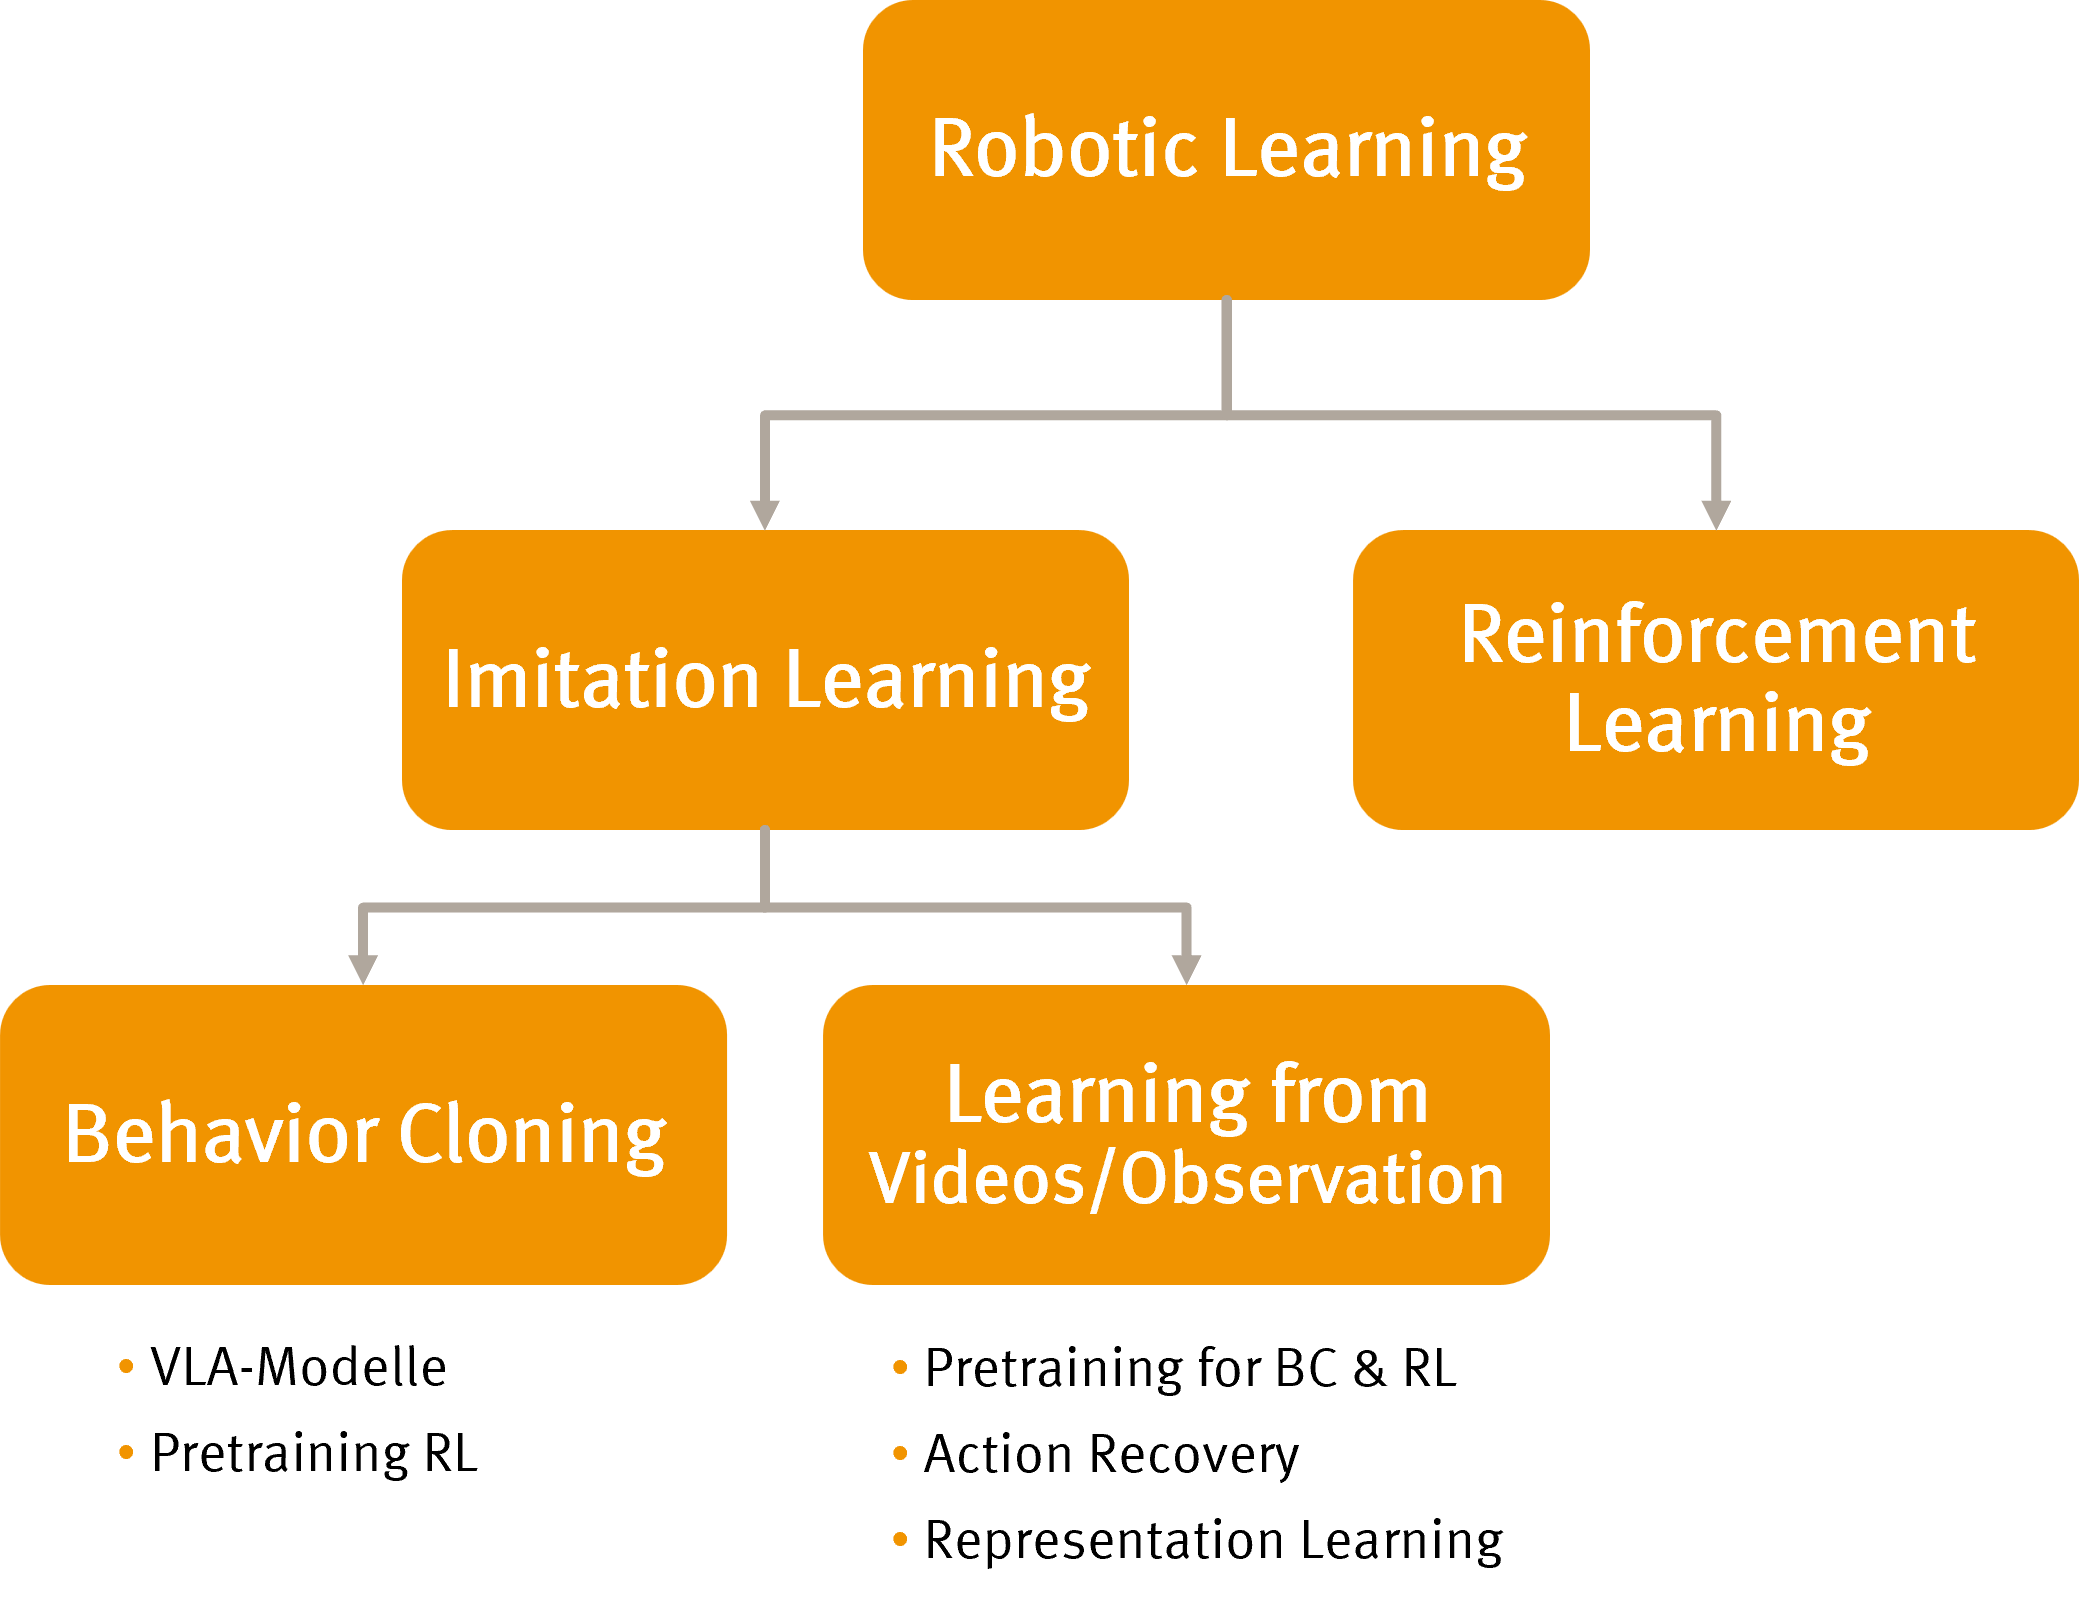
\includegraphics[width=0.6\linewidth]{./chapter3/media/OverviewRoboticLearning}
% 	\caption[Overview Robotic Learning]{Overview Robotic Learning}
% 	\label{fig:overviewroboticlearning}
% \end{figure}


% Methods from the \ac{LfV} paradigm can be used for action recovery, making unannotated video data applicable for \ac{BC} by recovering or estimating the underlying actions \cite{McCarthy_2025}. Furthermore, such methods can be employed to pretrain models for \ac{BC} or \ac{RL}, for example by learning expressive state and action representations through representation learning \cite{McCarthy_2025}.

% \ac{BC} is also widely used for training \ac{VLA} models and for pretraining \ac{RL} \ac{KM}s, for instance by learning components like value functions or reward models \cite{McCarthy_2025, Eze2024LearningBW}. In practice, \ac{BC} and \ac{LfV} are often combined to exploit the advantages of both approaches, enabling the use of large-scale unannotated data while maintaining the efficiency of supervised policy learning.







\section{Multi-Modal Models \& \acs{VLA} Models}
\label{sec:MultiModalApproachesVLAModels}
% Vision-Language-Action (VLA) models represent a recent frontier in robotic intelligence by jointly integrating visual perception, natural language understanding and robot action generation into a unified framework. These models enable robots to interpret visual environments, understand human instructions expressed in natural language and execute grounded robotic actions accordingly.

Multi-modal robotic learning aims to integrate several modalities, including visual observations, language instructions, robot states, tactile information and robot actions into a unified learning framework. The main objective is to improve task understanding, robustness and generalization across diverse environments and manipulation tasks \cite{rt12022arxiv, rt22023arxiv}. These approaches are considered an important step toward general-purpose robotic intelligence.


Multi-modal models that explicitly include robot actions are often called \acf{VLA} models, which jointly model visual perception, language understanding and robotic control. \ac{VLA} models extend Vision-Language Models by incorporating robot actions as an additional modality, enabling end-to-end policy learning from observations and natural language instructions. Their goal is to learn general-purpose robot policies capable of executing complex tasks across different environments \cite{Eze2024LearningBW}.


Another objective of \ac{VLA} models is to bridge the semantic gap between high-level multi-modal inputs and low-level robotic control \cite{Nvidia2025GR00TNA, Zhao2025CoTVLAVC, Li2024CogACTAF}. To achieve this, they learn shared representations across modalities such as language, vision (images, videos), robot states and actions and sometimes other modalities, like proprioception, touch or depth. Through large-scale training on multi-modal datasets, \ac{VLA} models align semantic understanding with motor behavior, allowing robots to generalize across diverse tasks and environments \cite{Eze2024LearningBW}.



\paragraph{General \acs{VLA} Architectural Overview}
\begin{figure}[!ht]
	\centering
	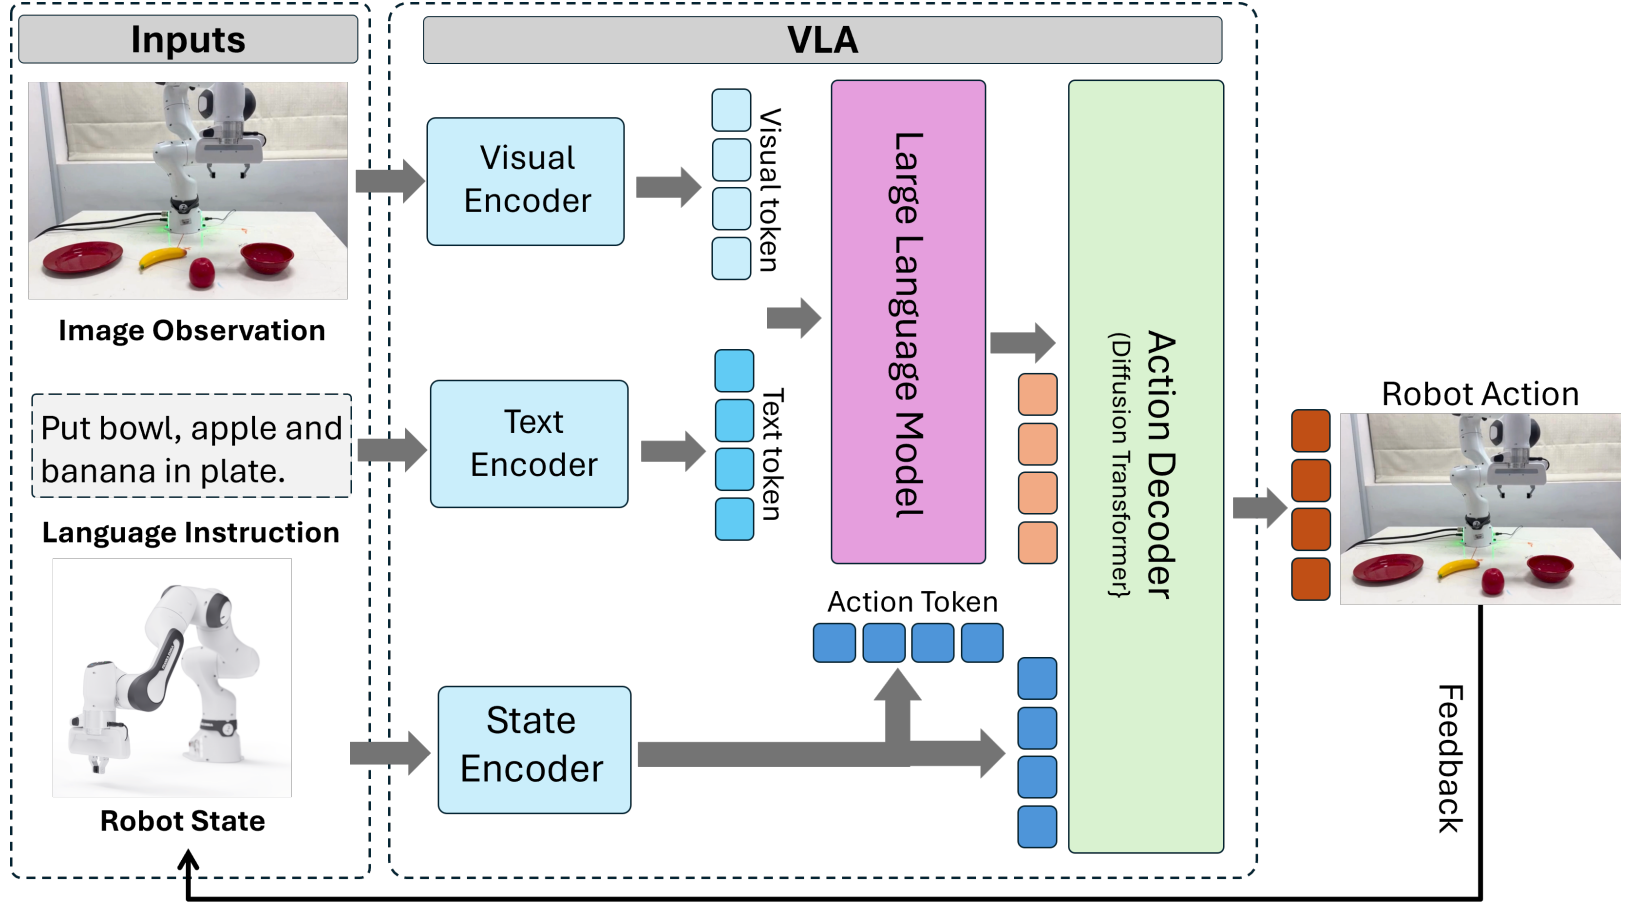
\includegraphics[width=1.0\linewidth]{./chapter6/media/VLAArchitecture}
	\caption[Vision-Language-Action Models: General overview of the Architecture]{Vision-Language-Action Models: General overview of the Architecture. Image source: \cite{Din2025VisionLA}.}
	\label{fig:VLAArchitecture}
\end{figure}

Figure \ref{fig:VLAArchitecture} illustrates the general architecture of a \ac{VLA} model for robotic manipulation \cite{Din2025VisionLA}. Such systems typically process three main inputs: a visual observation of the scene, a natural language instruction and the robot's internal state information. These inputs are encoded separately using Visual, Language and State Encoders to obtain modality-specific feature representations.

The resulting embeddings are then fused and aligned in one common embedding space within a \ac{LLM} or multi-modal transformer, which performs high-level semantic reasoning and generates a semantic representation of the task. Finally, this representation is combined with robot state features and passed to an Action Decoder, which predicts the sequence of robot actions or trajectories required to execute the commanded task. The Action Decoder can take various forms and is here illustrated as a Diffusion Policy, which directly generates actions based on the fused representation.

Technically, these systems combine advances in deep representation learning, multi-modal alignment and decision making, often leveraging transformer-based architectures trained with large-scale supervised or autoregressive objectives \cite{Din2025VisionLA}.




The mind map in Figure \ref{fig:VLAComponentsOverview} shows the main categories of Vision Encoders, Language Encoders and Action Decoders used in modern \ac{VLA} models. The listed architectures represent common design choices for multi-modal perception, semantic reasoning and robotic action generation in current large-scale robotic systems \cite{Din2025VisionLA}.

Some models appear under multiple encoder categories because they employ hybrid architectures that combine several pretrained backbones within a unified framework to improve visual representation quality, grounding capabilities and downstream manipulation performance.
\begin{figure}[!ht]
	\centering
	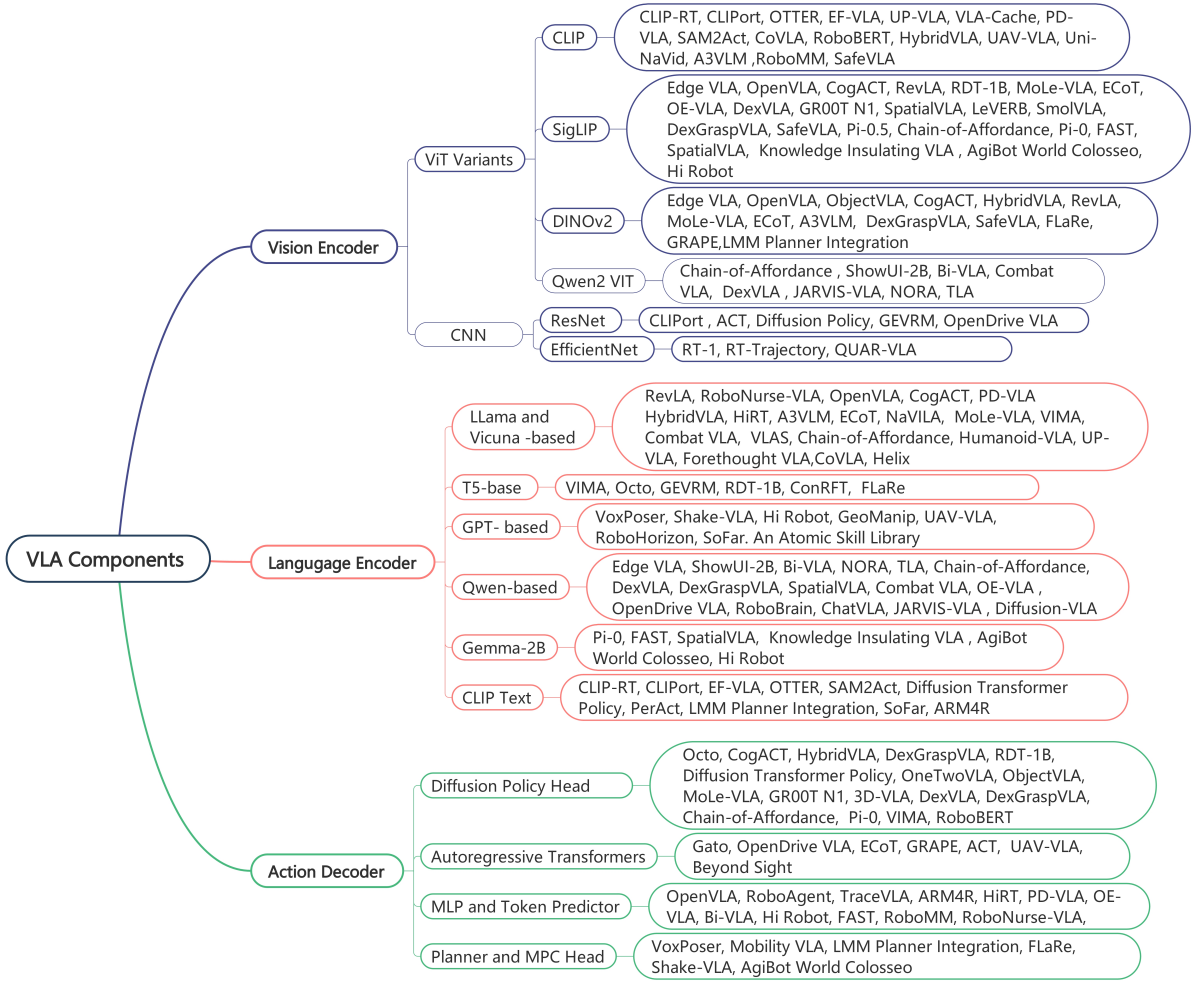
\includegraphics[width=1.0\linewidth]{./chapter6/media/VLAComponentsOverview}
	\caption[Vision-Language-Action Models: Overview of the components]{Vision-Language-Action Models: Overview of the components. Image source: \cite{Din2025VisionLA}.}
	\label{fig:VLAComponentsOverview}
\end{figure}






% Unlike traditional \ac{IL} approaches that are often specialized for a single task or embodiment, VLA models aim to support broad task generalization. 
% This includes robotic manipulation, navigation and human-robot interaction tasks, where the robot must reason about both the visual scene and the linguistic instruction before producing sequential control actions. 




\paragraph{Main VLA Architectural Paradigms}
\begin{figure}[!ht]
	\centering
	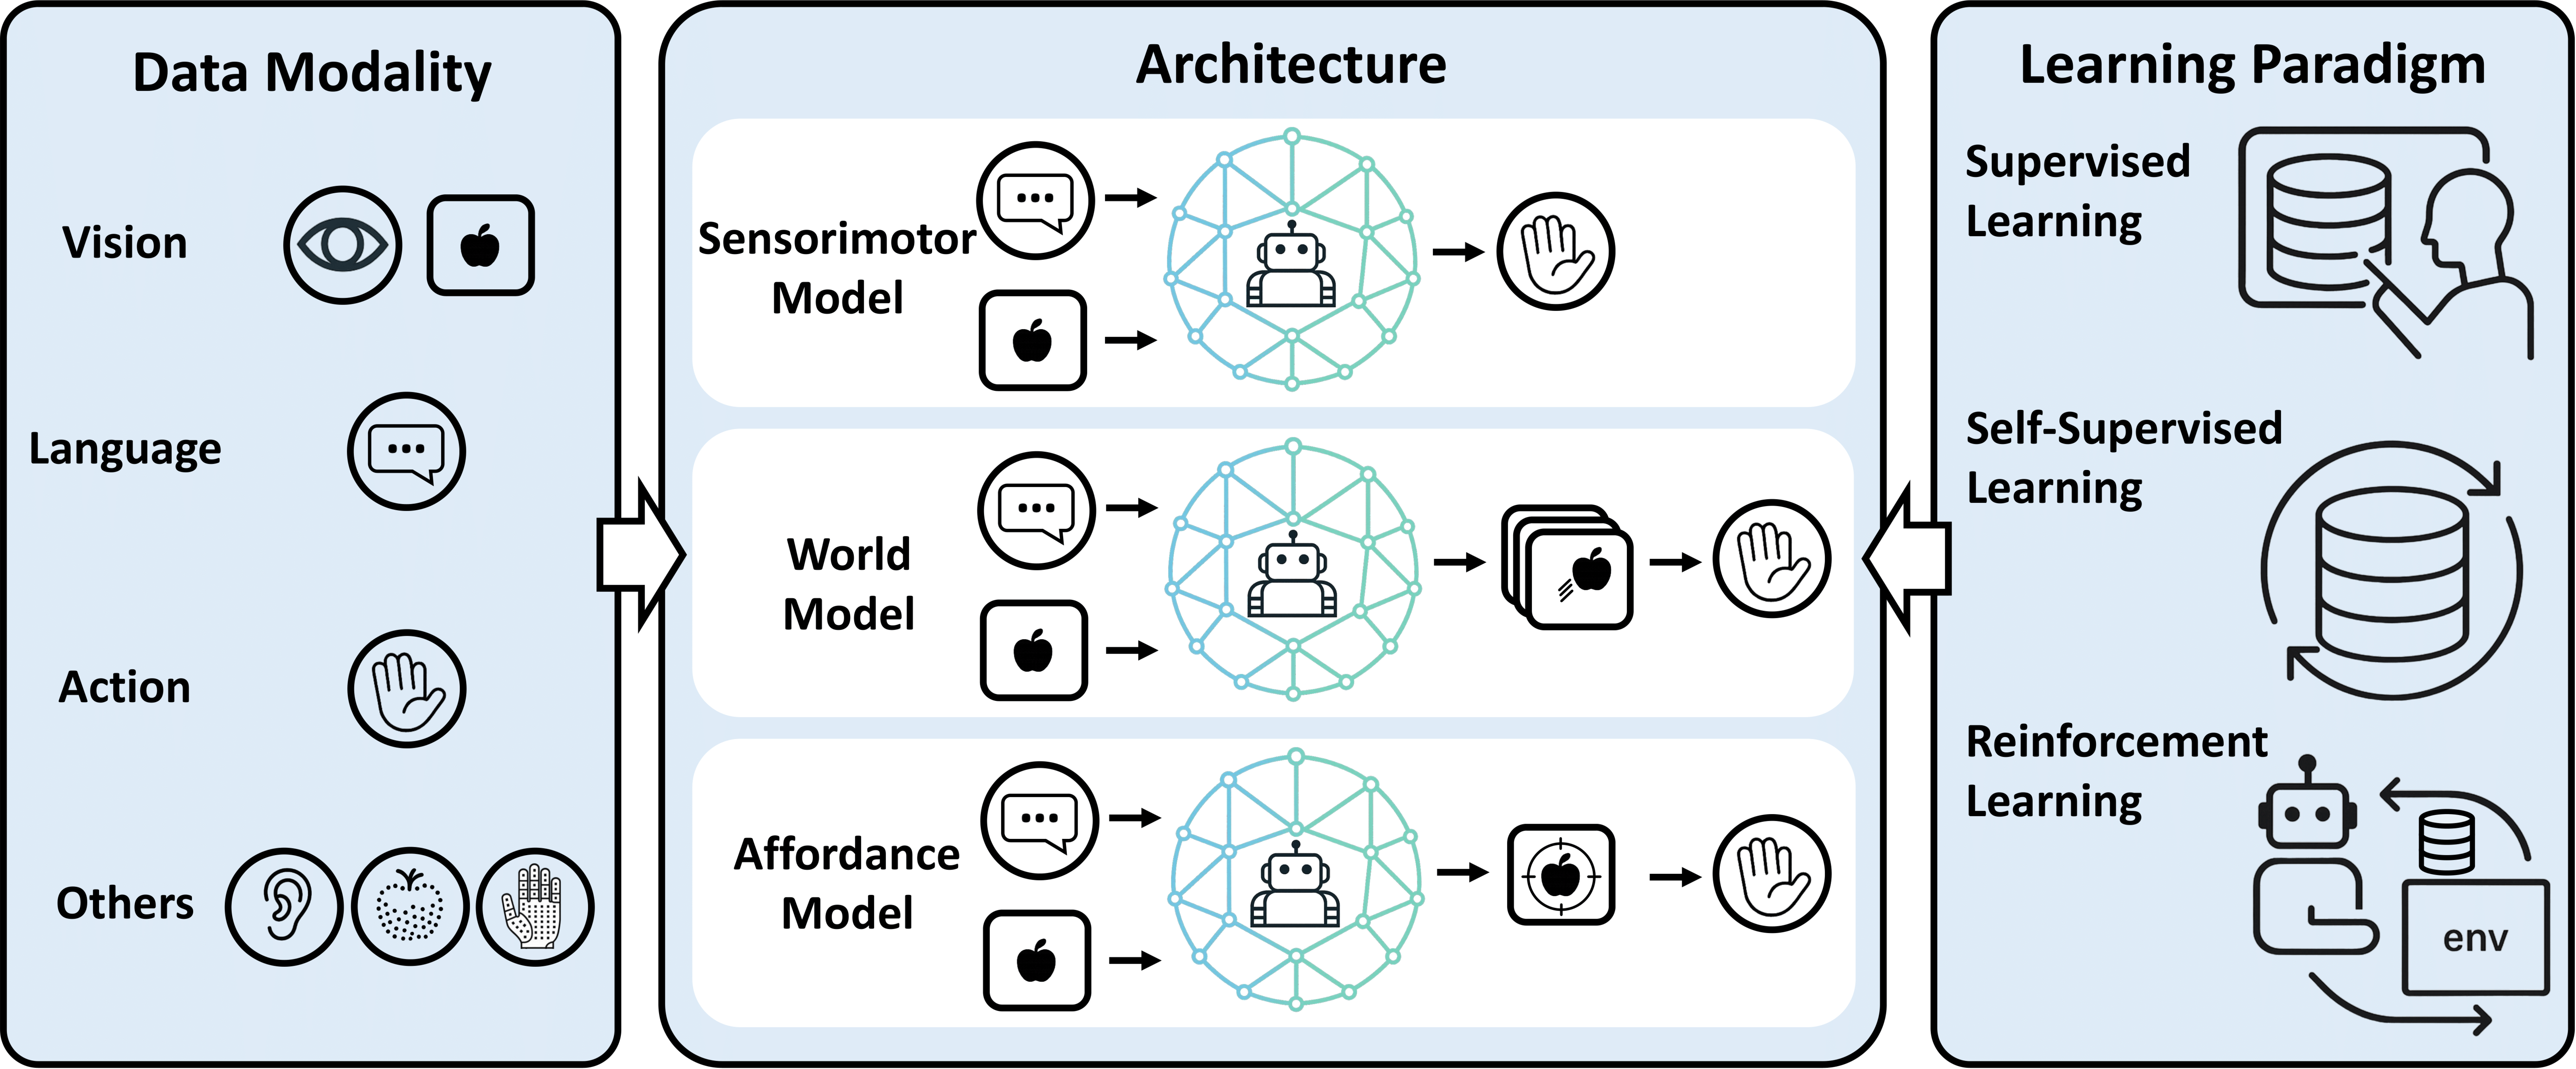
\includegraphics[width=1.0\linewidth]{./chapter6/media/VLAModalityArchitectureLearningParadigm.png}
	\caption[Vision-Language-Action Models: Modality, Architecture and Learning Paradigm]{Vision-Language-Action Models: Modality, Architecture and Learning Paradigm. Image source: \cite{Kawaharazuka2025VisionLanguageActionMF}.}
	\label{fig:VLAModalityArchitectureLearningParadigm}
\end{figure}

\ac{VLA} models encompass a broad range of architectural designs that differ in how perception, language understanding and robotic control are integrated. Learning paradigms also vary and include supervised learning, self-supervised learning and \ac{RL}, which can be combined in various ways.
\textcite{Kawaharazuka2025VisionLanguageActionMF} categorizes \ac{VLA} architectures into three main classes: sensorimotor models, world models and affordance-based models. Each class represents a different strategy for grounding multi-modal inputs into robotic actions and has its own architectures, see Figure \ref{fig:VLAModalityArchitectureLearningParadigm}.
% Most modern approaches combine advances in deep representation learning, multimodal alignment and sequential decision making, typically using transformer-based architectures trained on large-scale multimodal datasets.
\begin{itemize}
    \item \textbf{Sensorimotor Models:} Sensorimotor models jointly learn representations of visual observations, language instructions and robot actions within a unified policy model. These architectures directly map images and textual commands to robot actions and may employ either flat end-to-end policies or hierarchical structures that separate high-level reasoning from low-level control \cite{Kawaharazuka2025VisionLanguageActionMF}.
    \item \textbf{World Models:} Beyond direct policy learning, several alternative \ac{VLA} paradigms have emerged. World-model-based approaches learn the temporal dynamics of the environment by predicting future visual or latent states conditioned on actions and language inputs. These predicted future trajectories can then guide planning and action generation \cite{Kawaharazuka2025VisionLanguageActionMF}. 
    \item \textbf{Affordance-Based Models:} Another direction are affordance-based models, which predict task-relevant affordances or interaction regions from visual and language inputs before generating corresponding robot actions \cite{Kawaharazuka2025VisionLanguageActionMF}.
\end{itemize}

Together, these architectural strategies illustrate the ongoing shift from task-specific robotic policies toward more general-purpose, multi-modal robotic intelligence systems. \ac{VLA} models represent the recent frontier in robotic intelligence by jointly integrating visual perception, natural language understanding and robot action generation into a unified framework \cite{Kawaharazuka2025VisionLanguageActionMF}.
% Vision-Language-Action (VLA) models represent a recent frontier in robotic intelligence by jointly integrating visual perception, natural language understanding and robot action generation into a unified framework.




% Recent large-scale VLA systems further extend ideas from vision-language foundation models to embodied control by treating robot actions as another modality within a unified token-based prediction framework. This enables the transfer of semantic knowledge from internet-scale visual and language data to robotic policy learning, improving task flexibility and zero-shot generalization capabilities.


% \subsection{Comparison of approaches}
